\documentclass[12pt]{article}

%% Packages
\usepackage[margin=1in, top=0.75in]{geometry}
\usepackage[utf8]{inputenc}
\usepackage[T1]{fontenc}
\usepackage[usenames,dvipsnames]{xcolor}
\usepackage{amssymb, amsfonts, amsmath, mathrsfs, enumitem, tcolorbox, bbm, graphicx, fullpage, parskip, mathtools, float, amsthm}
\usepackage{tikz,sgame,bbm,todonotes, setspace, soul}
\usepackage[english]{babel}

\setcounter{tocdepth}{2}
% Links (and references)
\definecolor{linkblue}{RGB}{40, 50, 200}
\usepackage[colorlinks=true, allcolors={linkblue}]{hyperref}

%% Math operators
\newcommand*{\ones}{\text{\usefont{U}{bbold}{m}{n}1}}
\newcommand{\reals}{\mathbb{R}}
\newcommand{\rationals}{\mathbb{Q}}
\newcommand{\integers}{\mathbb{Z}}
\newcommand{\naturals}{\mathbb{N}}
\newcommand{\complex}{\mathbb{C}}
\newcommand{\normal}{\mathcal{N}}

% General math
\newcommand{\abs}[1]{\mathop{\left|#1\right|}} % absolute value
\newcommand{\inv}{^{-1}} % inverse
\let\oldST\st
\newcommand{\strikethrough}{\oldST}
\renewcommand{\st}{\;\text{s.t.}\;} % math operator for "such that"
\newcommand{\eg}{\emph{e.g.} }
\newcommand{\ie}{\emph{i.e.} }
\newcommand{\interior}{\mathop{\rm int}}

% Optimization
\newcommand{\argmax}{\mathop{\rm argmax}}
\newcommand{\argmin}{\mathop{\rm argmin}}
\newcommand{\opt}{^\star}
% Analysis, vector spaces, and topology
\newcommand{\set}[1]{\left\{#1\right\}} % set notation
\newcommand{\seq}[1]{_{#1}^{\infty}} % add sequence notiation to set (or to a summation symbol for series)
\newcommand{\setless}{\mathop{\backslash}} % A \ B notation
\newcommand{\pow}{\mathop{\mathcal{P}}} % power set
\newcommand{\im}{\mathop{\rm im}} % image
\newcommand{\spans}{\mathop{\rm span}} % span
\newcommand{\rank}{\mathop{\rm rank}} % rank
\newcommand{\topo}{\mathop{\mathcal{T}}} % topology
\newcommand{\cont}{\mathop{\bf C}} % continuously differentiable

% Matrices
\newcommand\colvector[1]{\begin{bmatrix}#1\end{bmatrix}}
\newcommand\rowvector[1]{\begin{bmatrix}#1\end{bmatrix}}
\newcommand\matrixc[1]{\begin{bmatrix}#1\end{bmatrix}}
\newcommand\matrixp[1]{\begin{pmatrix}#1\end{pmatrix}}
\newcommand\detmatrix[1]{\begin{vmatrix}#1\end{vmatrix}}
\newcommand\rankmatrix{\begin{bmatrix}I_r & \rvline & \mathbf{0}_1\\\hline \mathbf{0}_2 & \rvline & \mathbf{0}_3 \end{bmatrix}}

% Statistics
\newcommand{\cov}{\mathop{\rm cov}} % covariance
\newcommand{\corr}{\mathop{\rm corr}} % correlation
\newcommand{\expect}{\mathop{\mathbb{E}}} % expectation
\newcommand{\indep}{\perp \hspace{-1.4ex} \perp} % independence symbol
\newcommand{\distiid}{\mathop{\overset{\text{i.i.d.}}\sim}} % i.i.d.
\newcommand{\oversim}[1]{\mathop{\overset{\text{#1}}\sim}} % general text over \sim
\newcommand{\prob}{\mathbb{P}}
\newcommand{\mse}{\mathop{\rm MSE}}
\newcommand{\var}{\mathop{\rm Var}}
\newcommand{\sd}{\mathop{\rm sd}}
\newcommand{\se}{\mathop{\rm se}}
\newcommand{\bias}{\mathop{\rm bias}}
\newcommand{\toprob}{\overset{p}{\to}}
\newcommand{\toas}{\overset{a.s.}{\to}}
\newcommand{\todist}{\overset{d}{\to}}
\newcommand{\hyp}{\mathbb{H}}

% Economics
\newcommand{\choice}{\mathop{C_{\succsim}}} % choice correspondence

% Update existing operators
\let\oldExists\exists
\renewcommand{\exists}{\oldExists\;}
\let\oldForall\forall
\renewcommand{\forall}{\;\oldForall\;}
\let\oldEmptyset\emptyset
\renewcommand{\emptyset}{\mathop{\varnothing}}
\newcommand{\parl}{\left(}
\newcommand{\parr}{\right)}
\newcommand{\midbar}{\middle|}
\newcommand{\barl}{\left[}
\newcommand{\barr}{\right]}
\newcommand{\curll}{\left\{}
\newcommand{\curlr}{\right\}}


%% Presentation environments
% Proofs, counterexamples, and disproofs
\renewcommand\qedsymbol{$\openbox$}
\renewenvironment{proof}{{\raggedright \textit{\textbf{Proof.}}}}{\qed} % Proof
\newenvironment{pf}{\begin{proof}}{\end{proof}} % Proof (shorthand)

\newenvironment{disproof}{{\raggedright \textit{\textbf{Disproof.}}}}{$\qed$} % Disproof
\newenvironment{counterex}{{\raggedright \textit{\textbf{Counterexample.}}}}{} % Counterexample

% Theorem styles
\theoremstyle{plain}
\newtheorem{result}{Result}
\newtheorem{lemma}{Lemma}[section]
\newtheorem{assumption}{Assumption}[section]
\newtheorem{theorem}{Theorem}[section]
\newtheorem{proposition}{Proposition}[section]
\newtheorem{corollary}{Corollary}[section]
\newtheorem{axiom}{Axiom}[section]
\theoremstyle{definition}
\newtheorem*{example}{Example}
\newtheorem*{definition}{Definition}
\newtheorem*{exercise}{Exercise}
\newtheorem*{model}{Model}
\newtheorem*{proposition*}{Proposition}
\newtheorem*{model*}{Model}
\newtheorem*{solution}{Solution}
\newtheorem*{remark}{Remark}
\newtheorem*{question}{Question}
\newtheorem*{answer}{Answer}
\newtheorem*{algorithm}{Algorithm}

\newcommand{\blue}[1]{\textcolor{blue}{\emph{#1}}}
\newcommand{\red}[1]{\textcolor{red}{\emph{#1}}}




\newcommand{\gabe}[1]{\todo[inline,color=green!20!white]{\textbf{GS:} #1}}


%% Header
\makeatletter
\newcommand{\course}[1]{\def\@course{#1}}
\newcommand{\term}[1]{\def\@term{#1}}
\renewcommand{\title}[1]{\def\@entitle{#1}}
\renewcommand{\maketitle}{
    \begin{tcolorbox}[colframe=darkgray]
        \begin{center}
            \textbf{\@course} \\[0.25em]
            {\Large\textit{\@entitle}} \\[0.5em]
            Gabe Sekeres \\[0.5em]
            \@term
        \end{center}
    \end{tcolorbox}
    \vspace{1em}
}
\makeatother


%% Code
\usepackage{listings}
\usepackage{beramono}
\lstdefinelanguage{Julia}%
  {morekeywords={abstract,break,case,catch,const,continue,do,else,elseif,%
      end,export,false,for,function,immutable,import,importall,if,in,%
      macro,module,otherwise,quote,return,switch,true,try,type,typealias,%
      using,while},%
   sensitive=true,%
   alsoother={$},%
   morecomment=[l]\#,%
   morecomment=[n]{\#=}{=\#},%
   morestring=[s]{"}{"},%
   morestring=[m]{'}{'},%
   breaklines=true,%
}[keywords,comments,strings]%

\lstset{%
    language         = Julia,
    basicstyle       = \ttfamily,
    keywordstyle     = \bfseries\color{blue},
    stringstyle      = \color{magenta},
    commentstyle     = \color{ForestGreen},
    showstringspaces = false,
}






\title{Microeconomics I Notes}
\author{Gabe Sekeres \& Omar Andujar}
\course{ECON 6090}
\term{Fall 2024}
\begin{document}
\maketitle

\section*{Introduction}

We are creating this set of unified notes for ECON 6090: Microeconomics I, as taught at Cornell University in the Fall 2024 semester. Due to unforeseen departmental circumstances, this course was taught by six different professors (\href{https://easley.economics.cornell.edu/}{David Easley}, \href{https://philippkircher.com/}{Philipp Kircher}, \href{https://adamharris.phd/}{Adam Harris}, \href{https://sites.santafe.edu/~leb/}{Larry Blume}, \href{https://barseghyan.economics.cornell.edu/}{Levon Barseghyan}, and \href{https://www.mbattaglini.com/}{Marco Battaglini}). This structure necessarily created some confusion in notation and material, so these notes function as my attempt to create a universe of the material we learned.

We rely heavily on the notes created from Prof. Easley's course, which were originally compiled by \href{https://julienneves.com/}{Julien Manuel Neves} and subsequently updated by \href{https://ruqing-xu.github.io/}{Ruqing Xu} and \href{https://economics.cornell.edu/patrick-ferguson}{Patrick Ferguson}, as well as the excellent TA Sections curated by \href{https://economics.cornell.edu/yuxuan-ma}{Yuxuan Ma} and \href{https://dyson.cornell.edu/programs/graduate/graduate-student-directory/}{Feiyu Wang}. We additionally rely on notes and slides provided by Prof. Harris, slides provided by Prof. Blume, slides from \href{https://blogs.cornell.edu/odonoghue/}{Ted O'Donoghue} provided by Prof. Barseghyan, and notes provided by Prof. Battaglini. These notes are supplemented with the canonical \href{https://global.oup.com/academic/product/microeconomic-theory-9780195073409?cc=us&lang=en&}{Microeconomic Theory} textbook by \href{https://www.upf.edu/web/andreu-mas-colell}{Andreu Mas-Colell}, \href{https://mitsloan.mit.edu/faculty/directory/michael-whinston}{Michael Whinston}, and \href{https://www.hbs.edu/faculty/Pages/profile.aspx?facId=6466}{Jerry Green} (hereafter, MWG); \href{https://www.semanticscholar.org/paper/Utility-theory-for-decision-making-Fishburn/905a24a912171436e0abd3b5f1fdcb963e6f852f}{Utility Theory for Decision Making} by \href{https://en.wikipedia.org/wiki/Peter_C._Fishburn}{Peter Fishburn}; a classic analysis textbook, \href{https://store.doverpublications.com/products/9780486477664}{Foundations of Mathematical Analysis} by \href{https://condor.depaul.edu/~rjohnson/}{Richard Johnsonbaugh} and \href{https://www.mathgenealogy.org/id.php?id=12494}{W.E. Pfaffenberger}; and the excellent Mathematics notes provided by \href{https://www.takumahabu.com/Economics}{Takuma Habu}. All mistakes are our own.

We occasionally make reference to the Stanford ECON 202 notes, created by \href{https://www.gsb.stanford.edu/faculty-research/faculty/jonathan-levin}{Jonathan Levin}, \href{https://web.stanford.edu/~isegal/}{Ilya Segal}, \href{https://milgrom.people.stanford.edu/}{Paul Milgrom}, and \href{https://sites.google.com/site/ravijagadeesan/}{Ravi Jagadeesan}. This will mainly be if there exists intuition that we believe is helpful.

\paragraph{Notation.} A large part of this project is an attempt to unify the notation used by our separate professors. We default to the notation used in the Easley notes, then to MWG, and then use our own judgement. New definitions will have a word highlighted in \blue{blue}, and certain (named) theorems will be denoted in \red{red}. 

\paragraph{Structure.} The course (and these notes) are organized as follows. Prof. Easley taught an introduction to choice theory, Section~\ref{sec:easley}. Prof. Kircher taught consumer theory, Section~\ref{sec:kircher}. Prof. Harris taught producer theory, and some concepts of market failures, Section~\ref{sec:harris}. Prof. Blume introduced the theory of choice under uncertainty, Section~\ref{sec:blume}, and Prof. Barseghyan continued with theoretical applications for uncertainty and expected utility maximization, Section~\ref{sec:barseghyan}. Prof. Battaglini taught on information theory, Section~\ref{sec:battaglini}. We also include here exercises with solutions, divided into the various sections and sources. This is Section~\ref{sec:exercises}.

\paragraph{Contributions.} Gabe wrote Section~\ref{sec:easley}, and XXX. Omar wrote the section exercises and solutions in Section~\ref{sec:exercises}, and YYY. We are deeply grateful to everyone who read over these notes and suggested edits, especially our cohortmates 


\newpage
\section{Choice (Easley)}\label{sec:easley}

\subsection{Preference Theory}

\begin{assumption}
	Let $X$ be a finite set of objects. 
\end{assumption}

\begin{definition}
	Define $\succsim$, a \blue{preference relation} on $X$, as $x \succsim y \Longleftrightarrow x$ is \emph{at least as good as} $y$, for $x,y \in X$. $\succsim$ is a binary relation.
\end{definition}

\begin{definition}
	$x$ is \blue{strictly preferred} to $y$, denoted as $x \succ y$, if $x \succsim y$ and $y \not\succsim x$.
\end{definition}
\begin{definition}
	$x$ is \blue{indifferent} to $y$, denoted as $x \sim y$, if $x \succsim y$ and $y \succsim x$.
\end{definition}

\begin{definition}
	A preference relation $\succsim$ is \blue{complete} if $\forall x,y \in X$, either $x\succsim y$, $y \succsim x$, or both.
\end{definition}
\begin{definition}
	A preference relation $\succsim$ is \blue{transitive} if, $\forall x,y,z \in X$ where $x \succsim y$ and $y \succsim z$, $x \succsim z$.
\end{definition}
\begin{definition}
	A preference relation $\succsim$ is \blue{rational} if it is complete and transitive.
\end{definition}
\begin{remark}
	Prof. Easley takes some issues with this definition. The main issue is that there is an English word `rational' that has absolutely nothing to do with it. Hereafter, always read rational as `complete and transitive'.
\end{remark}

\begin{remark}
	These are all of the abstract concepts in choice theory! From here, we will apply them, and see what we can get. 
\end{remark}

\begin{definition}
	(Informal) Define a \blue{choice structure} $C\opt$ over subsets $B \subseteq X$ as $C\opt(B,\succsim) \coloneqq \{x \in B : x \succsim y \forall y \in B\}$.
\end{definition}
\begin{remark}
	Some direct implications:
	\begin{itemize}
		\item[(i)] If $x \in C\opt(B,\succsim)$ and $y \in C\opt(B,\succsim)$, then $x \sim y$.
		
		\item[(ii)] Suppose that $x \in B$, $x \not\in C\opt(B,\succsim)$, and $C\opt(B,\succsim) \ne \emptyset$. Then there exists $y \in B$ such that $y \succ x$. 
	\end{itemize}
\end{remark}

We will now formalize the above.

\begin{definition}
	Let the \blue{power set} of $X$, denoted $\mathcal{P}(X)$, be the set of all subsets of $X$. Note that since $X$ is finite, $\mathcal{P}(X)$ is finite.
\end{definition}

\begin{definition}
	(Formal) A correspondence $C\opt : \mathcal{P}(X) \rightrightarrows X$ is a \blue{choice correspondence} for some (not necessarily complete; not necessarily transitive) preference relation $\succsim$ if $C\opt(B) \subseteq B$ for all $B \subseteq X$.
\end{definition}
\begin{remark}
	This definition is from the Stanford notes -- I find it more intuitive than defining it the other way, but it requires divorcing the choice structure from the preference relation. Some intuition that's helpful for me: Easley's definition starts with the preference relation and then defines the choice correspondence, while Segal's definition starts with the choice correspondence and then applies it to a preference relation. They will (as we will see below) often be equivalent, but it's a subtle distinction. I will denote an arbitrary choice correspondence by $C\opt(\cdot)$ and one connected with a preference relation $\succsim$ by $C\opt(\cdot, \succsim)$.
\end{remark}

\begin{proposition}\label{prop:rational_choice_nonempty}
	If $\succsim$ is a rational preference relation on $X$, then
	\[
	C\opt : \mathcal{P}(X) \setminus \emptyset \to \mathcal{P}(X) \setminus \emptyset 
	\]
	In words, the associated choice correspondence to a rational preference relation is nonempty for nonempty inputs.
\end{proposition}
\begin{remark}
	The Easley notes define power sets slightly differently. This is unnecessary and (I feel) less intuitive.
\end{remark}
\begin{proof}
	Proof by induction on $n = |B|$. Suppose $|B| = 1$, so $B = \{x\}$ for some $x \in X$. Then by completeness, $x \succsim x$, and $C\opt(B,\succsim) = \{x\} \in \mathcal{P}(X) \setminus \emptyset$. Suppose next that for any $Y$ where $|Y| = n$, $C\opt(Y,\succsim)$ is nonempty. Take some arbitrary $B$, where $|B| = n + 1$. Define $B'\coloneqq B \setminus \{x\}$, and let $x'$ be an element of $C\opt(B',\succsim)$, which is nonempty by the inductive hypothesis. By completeness, either $x \succ x'$, $x' \succ x$, or $x \sim x'$. Case by case, we would have that $C\opt(B,\succsim) \in \curll\{x\},C\opt(B',\succsim),C\opt(B',\succsim) \cup \{x\}\curlr \subseteq \mathcal{P}(X)$, by transitivity.
\end{proof}

\begin{definition}
	$C\opt$ satisfies \blue{Sen's $\alpha$}, also known as \blue{independence of irrelevant alternatives}, if $x \in A \subseteq B$ and $x \in C\opt(B,\succsim)$ implies that $x \in C\opt(A,\succsim)$.
\end{definition}
\begin{remark}
	The classical example of a preference relation that violates Sen's $\alpha$ is `choosing the second-cheapest wine.' It should be fairly clear to see why this violates Sen's $\alpha$. Is it a rational preference relation?
\end{remark}

\begin{proposition}\label{prop:rational_alpha}
	If $\succsim$ is a rational preference relation, then $C\opt(\cdot,\succsim)$ satisfies Sen's $\alpha$.
\end{proposition}
\begin{proof}
	The result is trivially true if $A = B$. Suppose that $A \subset B$. Let $x \in C\opt(B,\succsim)$. Then $x \succsim y$ for all $y \in B$. In particular, if $y \in A \subseteq B$, then $x \succsim y$. Thus, $x \in C\opt(A,\succsim)$.
\end{proof}

\begin{definition}
	$C\opt$ satisfies \blue{Sen's $\beta$}, also known as \blue{expansion consistency}, if $x,y \in C\opt(A,\succsim)$, $A \subseteq B$, and $y \in C\opt(B,\succsim)$ implies that $x \in C\opt(B,\succsim)$.
\end{definition}

\begin{remark}
	I couldn't find a classical example violating Sen's $\beta$, but a simple one is as follows: assume that the waiter offers you French or Italian wine. You are indifferent between them, but then they remember that they also have California wine. You say 	`in that case, I'll have the French wine'. Again, this directly violate's Sen's $\beta$, but is it rational? Why or why not?
\end{remark}

\begin{proposition}\label{prop:rational_beta}
	If $\succsim$ is a rational preference relation, then $C\opt(\cdot,\succsim)$ satisfies Sen's $\beta$.
\end{proposition}
\begin{proof}
	Let $x,y \in C\opt(A,\succsim)$, $A \subseteq B$, and $y \in C\opt(B,\succsim)$. Since $x \in C\opt(A,\succsim)$, we have $x \succsim y$ since $y \in A$. Since $y \in C\opt(B,\succsim)$, we have $y\succsim z$ for all $z \in B$. By transitivity, $x \succsim y$ and $y \succsim z$ implies that $x \succsim z$ for all $z \in B$, so $x\in C\opt(B,\succsim)$. 
\end{proof}

\begin{definition}
	$C\opt$ satisfies \blue{Houthaker's weak axiom of revealed preference} (often called either \blue{HWARP} or \blue{HARP}) if for all $A,B \in \mathcal{P}(X)$ if $x,y \in A \cap B$, $x \in C\opt(A,\succsim)$ and $y \in C\opt(B,\succsim)$, then $x \in C\opt(B,\succsim)$ and $y \in C\opt(A,\succsim)$.
\end{definition}

\begin{proposition}\label{prop:alpha_beta_hwarp}
	$C\opt : \mathcal{P} \rightrightarrows X$ satisfies Sen's $\alpha$ and $\beta$ if and only if it satisfies Houthaker's weak axiom of revealed preference.
\end{proposition}
\begin{proof}
	
	\begin{itemize}
		\item[(i)] ($\alpha + \beta \Longrightarrow $ HWARP) Suppose $x,y \in A \cap B \subseteq \mathcal{P}(X)$, $x \in C\opt(A,\succsim)$, and $y \in C\opt(B,\succsim)$. By Sen's $\alpha$, both $x$ and $y$ are in $C\opt(A \cap B,\succsim)$. Then by Sen's $\beta$, $x \in C\opt(B,\succsim)$ and $y \in C\opt(A,\succsim)$.
		
		\item[(ii)] (HWARP $\Longrightarrow \beta$) Say $x,y \in C\opt(A,\succsim)$, $A \subseteq B$ and $y \in C\opt(B,\succsim)$. Because $A = A \cap B$, $x,y \in C\opt(A \cap B,\succsim)$. Applying HWARP, we have that $x \in C\opt(B,\succsim)$.
		
		\item[(iii)] (HWARP $\Longrightarrow \alpha$) Say $x \in A \subseteq B$ and $x \in C\opt(B,\succsim)$. Suppose $x \not\in C\opt(A,\succsim)$. Then by Proposition~\ref{prop:rational_choice_nonempty}, there exists $y \in C\opt(A,\succsim)$. Note that $x,y \in A = A \cap B$, $x \in C\opt(B,\succsim)$ and $y \in C\opt(A,\succsim)$. By HWARP, $x \in C\opt(A,\succsim)$, which is a contradiction.
	\end{itemize}
\end{proof}

\begin{proposition}\label{prop:hwarp_alpha_beta_equiv}
	The following are equivalent for $C\opt(\cdot,\succsim)$, where $C\opt: \mathcal{P}(X) \to \mathcal{P}(X)$
	\begin{itemize}
		\item[(i)] $\succsim$ is rational
		\item[(ii)] $C\opt$ satisfies Sen's $\alpha$ and $\beta$
		\item[(iii)] $C\opt$ satisfies HWARP
	\end{itemize}
\end{proposition}
\begin{proof}
	(ii) and (iii) are equivalent by Proposition~\ref{prop:alpha_beta_hwarp}. (i) $\Longrightarrow$ (ii) is given by Propositions~\ref{prop:rational_alpha} and \ref{prop:rational_beta}. Finally, (iii) $\Longrightarrow$ (i) is given below, in the proof of Proposition~\ref{prop:warp_rationality}.
\end{proof}

\subsection{Observed Choice}

Recall the formal definition of choice correspondences above. We will now add some more structure to that definition.

\begin{definition}
	For $\mathcal{B}$ a collection of subsets of $X$, $(\mathcal{B},C)$ is called a \blue{choice structure} if $C(B) \subseteq B$ and $C(B) = \emptyset \Longleftrightarrow B = \emptyset$ for all $B \in \mathcal{B}$.
\end{definition}

\begin{definition}
	The choice structure $(\mathcal{B},C)$ satisfies the \blue{weak axiom of revealed preference} (\blue{WARP}) if for all $A,B \in \mathcal{B}$ where $x$ and $y$ are in both $A$ and $B$, $x \in C(A)$, and $y\in C(B)$, then $x \in C(B)$ and $y \in C(A)$.\footnote{Note the difference in wording from before -- we cannot have as a condition that $x,y \in A \cap B$ as $A \cap B$ is not necessarily in $\mathcal{B}$.}
\end{definition}
\begin{remark}
	When $\mathcal{B} = \mathcal{P}(X)$, WARP is the same as HWARP.
\end{remark}
\begin{definition}
	Given a choice structure $(\mathcal{B},C)$, the \blue{revealed preference relation} $\succsim\opt$ is defined such that $x \succsim\opt y$ if $\exists B \in \mathcal{B}$ such that $x,y \in B$ and $x \in C(B)$.
\end{definition}
\begin{proposition}\label{prop:warp_rationality}
	Suppose that $X$ is finite and $\mathcal{B} = \mathcal{P}(X)$. If $(\mathcal{B},C)$ satisfies WARP then the revealed preference relation that it induces, $\succsim\opt$ is rational and $C(B) = C\opt(B,\succsim\opt)$ for all $B \in \mathcal{B}$.
\end{proposition}
\begin{proof}
	If $\mathcal{B} = \mathcal{P}(X)$ and $(\mathcal{B},C)$ is a choice structure, then $C(Y)$ is defined as nonempty for every $Y = \{x,y\} \subseteq X$. This implies that $x \succsim\opt y$ or $y \succsim\opt x$ for all $x,y \in X$, so $\succsim\opt$ is complete.
	
	Suppose $x\succsim\opt y$ and $y \succsim\opt z$. Then there exists $A \subseteq X$ containing $x$ and $y$ such that $x \in C(A)$; and $B\subseteq X$ containing $y$ and $z$ such that $y \in C(B)$. Moreover, $\{x,y,z\} \subseteq \mathcal{B}$ and $C(\{x,y,z\})$ is nonempty. Suppose $y \in C(\{x,y,z\})$. Then by WARP, $x \in C(\{x,y,z\})$. Suppose $z \in C(\{x,y,z\})$. Then again by WARP, $y \in C(\{x,y,z\})$ and thus $x \in C(\{x,y,z\})$. In any case, $x \in C(\{x,y,z\})$ implies that $x \succsim\opt z$, so $\succsim\opt$ is transitive.
	
	Let $x$ be an element of $C\opt(B,\succsim\opt)$. Then $x \succsim\opt y \forall y \in B$. Since $C(B)$ is nonempty, we have that $z \in C(B)$ for some $z$. By $x \succsim\opt z$, there exists $A \in \mathcal{B}$ such that $x,z \in A$ and $x \in C(A)$. Therefore by WARP, $x \in C(B)$. Conversely, suppose $x \in C(B)$. Then $x \succsim\opt y$ for all $y \in B$, and so $x \in C\opt(B,\succsim\opt)$.
\end{proof}

\begin{remark}
	A stronger version of Proposition~\ref{prop:warp_rationality} exists, though we do not present the proof here:
\end{remark}
\begin{proposition}\label{prop:warp_rationality_3}
	Suppose that $X$ is finite and for all $Y \subseteq X$ where $|Y| \le 3$, $Y \in \mathcal{B}$. If $(\mathcal{B},C)$ satisfies WARP then the revealed preference relation that it induces, $\succsim\opt$ is rational and $C(B) = C\opt(B,\succsim\opt)$ for all $B \in \mathcal{B}$.
\end{proposition}

\begin{remark}
	This does not hold for anything less strong than 3. Consider the following counterexample: Suppose $X = \{x,y,z,w\}$ and $\mathcal{B} = \{\{x,y\},\{y,z\},\{z,w\},\{w,x\}\}$. Let $C$ be defined by:
	\[
	C(\{x,y\}) = \{x,y\} \quad ;\quad C(\{y,z\}) = \{y,z\} \quad ;\quad C(\{z,w\}) = \{z,w\} \quad ;\quad C(\{w,z\}) = \{x\} 
	\]
	Because no pair of elements of $X$ are both in two elements of $\mathcal{B}$, WARP is vacuously satisfied. But neither $x \succsim\opt z$ or $z \succsim\opt x$, so $\succsim\opt$ is incomplete. We can also show that it is intransitive (how?). Moreover, if we extend $C$ to the family of all two-element subsets of $X$, such that everything except for $\{w,x\}$ is mapped to itself (and $C(\{w,z\}) = \{x\}$), $\succsim\opt$ is complete but remains intransitive.
\end{remark}

\subsection{Incomplete Preferences}

\begin{definition}
	$\succ$ is a \blue{strict partial order} if (i) for any $x,y \in X$, if $x \succ y$, then $y \not\succ x$, and (ii) $\succ$ is transitive.
\end{definition}
\begin{remark}
	Note that we are explicitly not defining $\sim$ as $x \sim y$ if $x \not\succ y$ and $y \not\succ x$. The two elements could be incomparable, we do not assume completeness here.
\end{remark}

\begin{proposition}\label{prop:partial_order}
	Define choice by
	\[
	C\opt(A,\succ) \coloneqq \{x \in A : \forall y \in A, y\not\succ x\}
	\]
	where $\succ$ is a strict partial order. Then $C$ satisfies Sen's $\alpha$ but not Sen's $\beta$.
\end{proposition}
\begin{proof}
	
	\begin{itemize}
		\item[(i)] Suppose $x \in A \subseteq B$ and $x \in C(B,\succ)$. Then there does not exist $y \in B$ such that $y \succ x$. It follows that no such $y$ exists in $A \subseteq B$ either, so $x \in C(A,\succ)$.
		
		\item[(ii)] Suppose that $x,y \in C(A,\succ)$, $A \subseteq B$, $y \in C(B,\succ)$, and there is some $z \succ x$ in $B$ such that $y$ and $z$ are incomparable. Then the hypotheses of Sen's $\beta$ are satisfied, but $x \not\in C(B,\succ)$.
	\end{itemize}
\end{proof}

\subsection{WARP and the Slutsky Matrix}

We will make the following assumptions throughout:

\begin{assumption}\label{ass:consumer_struc}
	We have (i) $L$ commodities, $x \coloneqq (x_1,\dots,x_L) \in \reals^L_+$; (ii) prices $p \coloneqq (p_1,\dots,p_L) \in \reals^L_{++}$; (iii) wealth $w > 0$; and (iv) budget set $B_{p,w} \coloneqq \{x \in \reals^L_+ : p\cdot x \le w\}$.
\end{assumption}

\begin{definition}
	We define the \blue{Walrasian demand function} (also sometimes called the \blue{Marshallian demand function}) by $x : \reals^L_{++} \times \reals_{++} \to \reals^L_+$, where $x(p,w)$ is the consumer's choice at prices $p$ and wealth $w$. Note that $(p,w)$ may not uniquely specify a value. In that case, we have the \blue{Walrasian (Marshallian) demand correspondence}, $X: \reals^L_{++} \times \reals_{++} \rightrightarrows \reals^L_+$.
\end{definition}

\begin{assumption}\label{ass:demand_assumptions}
We will almost always make the following assumptions on $x$:
\begin{itemize}
	\item[(i)] $x(p,w)$ is homogeneous of degree 0, meaning that
	\[
	x(\alpha p ,\alpha w) = x(p,w) \text{ for all } (p,w) \in \reals^L_{++} \times \reals_{++} \text{ and } \alpha > 0
	\]
	\item[(ii)] $x(p,w)$ satisfies Walras' Law: $p \cdot x(p,w) = w$ for all $(p,w) \in \reals^L_{++} \times \reals_{++}$
\end{itemize}
\end{assumption}
\begin{proposition}\label{prop:walras_law_choice_structure}
	Let $\mathcal{B}^W \coloneqq \{B_{p,w} : (p,w) \in \reals^L_{++} \times \reals_{++}\}$ and $C_x(B_{p,w}) \coloneqq \{x(p,w)\}$, and let $x$ be homogeneous of degree 0 and satisfy Walras' Law. Then $(\mathcal{B}^W,C_x)$ is a choice structure.
\end{proposition}
\begin{proof}
	We want to show that $C_x(B_{p,w})$ is a uniquely-defined nonempty subset of $B_{p,w}$ for all $B_{p,w} \in \mathcal{B}^W$. That $C_x(B_{p,w})$ is nonempty follows from the definition of $x$ as a function (or correspondence). Homogeneity of degree 0 implies that for $B_{p,w} = B_{\alpha p,\alpha w}$, $C_x(B_{p,w}) = C_x(B_{\alpha p,\alpha w})$. Walras' Law implies that $C_x(B_{p,w}) \subseteq B_{p,w}$.
\end{proof}

\begin{definition}
	In the context of consumer choice, $x(p,w)$ satisfies the \blue{weak axiom of revealed preferences} (\blue{WARP}) if the following holds: If $(p,w),(p',w') \in \reals^L_{++} \times \reals_{++}$ are such that $p' \cdot x(p,w) \le w'$ and $x(p',w') \ne x(p,w)$, then $p\cdot x(p',w') > w$.
\end{definition}
\begin{remark}
	Basically, if the consumer ever chooses $x'$ when $x$ is available, then there's no way that both $x$ and $x'$ could be available and $x$ would be chosen.
\end{remark}
\begin{definition}
	A \blue{Slutsky compensated price change} is a price change from $p$ to $p'$ accompanied by a change in wealth from $w$ to $w'$ that makes the old bundle just affordable. That is, such that $p' \cdot x(p,w) = w'$.
\end{definition}

\begin{proposition}
	\red{(Law of Compensated Demand)} Suppose that consumer demand $x(p,w)$ is homogeneous of degree 0 and satisfies Walras' Law. Then $x(p,w)$ satisfies WARP if and only if for any compensated price change from $(p,w)$ to $(p',w') \coloneqq (p',p' \cdot x(p,w))$ we have
	\[
	(p' - p)\cdot (x(p',w') - x(p,w)) \le 0
	\] 
	with strict inequality if $x(p',w') \ne x(p,w)$.
\end{proposition}
\begin{proof}
	By WARP, $p \cdot x(p',w') \ge p \cdot x(p,w) = w$, with strict inequality if and only if $x(p,w) \ne x(p',w')$. By Walras' Law, we have that $p'\cdot x(p',w') = p'\cdot x(p,w) = w'$. Subtracting, we get
	\[
	(p - p') \cdot x(p',w') \ge (p - p')\cdot x(p,w) \Longrightarrow (p' - p) \cdot (x(p',w') - x(p,w)) \le 0
	\]
	Conversely, say that $(p' - p) \cdot (x(p',w') - x(p,w)) \le 0$. Then we have that
	\[
	p' \cdot x(p',w') - p' \cdot x(p,w) - p \cdot (x(p',w') - x(p,w)) \le 0 \Longrightarrow p \cdot x(p',w') > w
	\]
	since $p' \cdot x(p',w') < p' \cdot x(p,w)$. The case of strict inequality is analogous.
\end{proof}

\begin{proposition}\label{prop:law_of_demand}
	Let $x : \reals^L_+ \times \reals_+ \to \reals^L_+$ be continuously differentiable. Then
	\[
	\frac{\partial x_j(p,w)}{\partial p_j} + x_j(p,w) \frac{\partial x_j(p,w)}{\partial w} \le 0
	\]
\end{proposition}
\begin{proof}
	Assume that $p$ changes solely in $p_j$, by $\Delta p_j > 0$, and let $\Delta w$ be the compensating change in wealth, as above. Let $\Delta x \coloneqq x(p',w') - x(p,w)$. Then by the Law of Compensated Demand, we have that
	\[
	\Delta p_j (x_j(p',w') - x_j(p,w)) \le 0 \Longrightarrow \frac{x_j(p',w') - x_j(p,w)}{\Delta p_j} \le 0
	\]
	Adding and subtracting $x_j(p',w)$, this becomes
	\[
	\frac{x_j(p',w) - x_j(p,w)}{\delta p_j} + \frac{x_j(p',w') - x_j(p',w)}{\Delta p_j} \le 0
	\]
	Using the fact that $\Delta w = \Delta p_j x_j(p,w)$, we get that
	\[
	\frac{x_j(p',w) - x_j(p,w)}{\delta p_j} + x_j(p,w)\frac{x_j(p',w') - x_j(p',w)}{\Delta w} \le 0
	\]
	Taking the limit as $\Delta p_j \searrow 0$, which implies that $\Delta w \searrow 0$ and $p' \to p$), and using the fact that $x$ is continuously differentiable, this becomes
	\[
	\frac{\partial x_j(p,w)}{\partial p_j} + x_j(p,w) \frac{\partial x_j(p,w)}{\partial w} \le 0
	\]
\end{proof}

\begin{definition}
	The \blue{Slutsky matrix} is the matrix of the partials defined above:
	\begin{align*}
		S(p,w) &\coloneqq D_p x(p,w) + D_w x(p,w) x(p,w)^T \\
		&= \matrixc{\frac{\partial x_1}{\partial p_1} + x_1 \frac{\partial x_1}{\partial w} & \cdots & \frac{\partial x_1}{\partial p_L} + x_L \frac{\partial x_1}{\partial w} \\ \vdots && \vdots \\\frac{\partial x_L}{\partial p_1} + x_1 \frac{\partial x_L}{\partial w} & \cdots & \frac{\partial x_L}{\partial p_L} + x_L \frac{\partial x_L}{\partial w} }
	\end{align*}
\end{definition}

\begin{proposition}\label{prop:slutsky_nsd}
	$S(p,w)$ is negative semi-definite.
\end{proposition}
\begin{proof}
	Let $dp \coloneqq (dp_1,\dots,dp_L)$ be an arbitrary element of $\reals^L$. Then for all $i$, we have that
	\begin{align*}
		dx_i &= \frac{\partial x_i}{\partial p_1}dp_1 + \cdots + \frac{\partial x_i}{\partial p_L}dp_L + \frac{\partial x_i}{\partial w}x_1(p,w)dp_1 + \cdots + \frac{\partial x_i}{\partial w}x_L(p,w)dp_L \\
		\Longrightarrow dx &= (D_px(p,w) + D_wx(p,w) x(p,w)^T) dp
	\end{align*}
	By WARP, $dp \cdot dx \le 0$, meaning that
	\[
	dp^T (D_px(p,w) + D_wx(p,w) x(p,w)^T) dp \le 0
	\]
	Thus, $S(p,w)$ is negative semi-definite, since $dp$ is arbitrary.
\end{proof}


\subsection{Consumer Choice from $\succsim$}

\begin{assumption}
	As before, let $X \coloneqq \reals^L_+$. 
\end{assumption}
\begin{definition}
	A \blue{utility function} representing $\succsim$ on $X$ is a function $u: X \to \reals$ such that for all $x,y \in X$:
	\[
	x \succsim y \Longleftrightarrow u(x) \ge u(y)
	\]
\end{definition}

\begin{proposition}
	If $u: X \to \reals$ represents $\succsim$ on $X$ and $f: \reals \to \reals$ is strictly increasing, then $f \circ u$ represents $\succsim$.
\end{proposition}
\begin{proof}
	\[
	x \succsim y \Longleftrightarrow u(x) \ge u(y) \Longleftrightarrow (f\circ u)(x) \ge (f\circ u)(y)
	\]
\end{proof}

\begin{remark}
	Lexicographic preferences, defined on $\reals^2$ by
	\[
	(x_1,x_2) \succsim (y_1,y_2) \Longleftrightarrow x_1 > y_1 \text{ or } x_1 = y_1 \text{ and } x_2 \ge y_2
	\]
	are rational but cannot be represented by a utility function. Why is that?
\end{remark}

\begin{definition}
	The following mathematical concepts will be useful to us:
	\begin{itemize}
		\item[(i)] The \blue{upper contour set}, $R(x) \coloneqq \{y \in X : y \succsim x\}$, is the set of all bundles that are at least as good as $x$. Denote its complement by $P^{-1}(x)$.
		
		\item[(ii)] The \blue{lower contour set}, $R^{-1}(x) \coloneqq \{y \in X : x \succsim y\}$, is the set of all bundles that $x$ is at least as good as. Denote its complement by $P(x)$.
	\end{itemize}
\end{definition}

\begin{definition}
	The preference relation $\succsim$ on $X$ is \blue{continuous} if $R(x)$ and $R^{-1}(x)$ are closed subsets of $X$ for all $x \in X$.
\end{definition}

\begin{remark}
	Lexicographic preferences are not continuous. Can you show why?
\end{remark}
\begin{proposition}\label{prop:debreu}
	\red{(Debreu's Theorem)} Suppose a preference relation $\succsim$ on $X$ is rational and continuous. Then there is a continuous utility function representing $\succsim$.
\end{proposition}
\begin{proof}
	(Sketch) We will sketch this proof assuming that $\succsim$ satisfy strong monotonicity (defined below), which is not necessary but makes the proof easier. Choose any $x \in X$. By strong monotonicity, $x \succsim 0$. Let $e = (1,1)$. By strong monotonicity, $\exists \alpha \in \reals_+$ such that $\alpha e \succ x$. By strong monotonicity, $\exists \alpha : X \to \reals_+$ such that $\alpha(x)e\sim x \forall x \in X$. 
	
	We claim that $\alpha(\cdot)$ represents $\succsim$. First, suppose that $\alpha(x) \ge \alpha(y)$. Then $\alpha(x)e \succsim \alpha(y)e$ by strict monotonicity, and by transitivity we have that $x \sim \alpha(x)e \succsim \alpha(y)e \sim y \Longrightarrow x \succsim y$. Conversely, assume that $x\succsim y$. Then $\alpha(x)e \sim x \succsim y \sim \alpha(y)e$, so $\alpha(x)e\succsim \alpha(y)e$ by transitivity, and $\alpha(x) \ge \alpha(y)$ by strict monotonicity.
\end{proof}

\begin{definition}
	The preference relation $\succsim$ is \blue{monotone} if for all $x,y \in X$, $x \ge y \Longrightarrow x\succsim y$. It is \blue{strictly monotone} if $x \ge y$ and $x \ne y$ implies that $x \succ y$. Note that the latter implies the former.
\end{definition}

\begin{definition}
	The preference relation $\succsim$ is \blue{locally non-satiated} if for every $x \in X$ and for every $\varepsilon > 0$, there exists $y \in X$ such that $\|x - y\| \le \varepsilon$ and $y \succ x$. Note that strict monotonicity implies local non-satiation.
\end{definition}
\begin{remark}
	We assumed earlier that $X = \reals^L_+$. This concept can be extended to any metric space, replacing the norm with the space's distance function.  
\end{remark}
\begin{definition}
	The preference relation $\succsim$ on $X$ is \blue{convex} if for all $x,y,z\in X$ and all $\alpha \in [0,1]$, $y \succsim x$ and $z \succsim x$ implies that $\alpha y + (1-\alpha)z \succsim x$.
	
	It is \blue{strictly convex} if for all $x,y,z \in X$ and all $\alpha \in (0,1)$, $y \ne z$, $y \succsim x$, and $z \succsim x$ imply that $\alpha y + (1-\alpha)z \succ x$.
\end{definition}

\begin{remark}
	Preferences are convex if and only if $R(x)$ is convex for every $x \in X$. Can you prove this?
\end{remark}

\begin{definition}
	The function $u: X \to \reals$ is \blue{quasiconcave} if for all $x,y \in X$ and any $\alpha \in [0,1]$,
	\[
	u(\alpha x + (1-\alpha)y) \ge \min\{u(x),u(y)\}
	\]
	The function $u: X \to \reals$ is \blue{concave} if for all $x,y \in X$ and any $\alpha \in [0,1]$,
	\[
	u(\alpha x + (1-\alpha)y) \ge \alpha u(x) + (1-\alpha)u(y)
	\]
	Strict quasiconcavity and strict concavity are defined analogously, restricting $\alpha$ to $(0,1)$, requiring that $x \ne y$, and replacing weak inequalities with strict ones.
\end{definition}
\begin{proposition}\label{prop:quasiconcave_convex}
	$u$ representing $\succsim$ is quasiconcave if and only if $\succsim$ is convex.
\end{proposition}
\begin{proof}
	Assuming quasiconcavity, $y,z \succsim z \Longrightarrow u(y),u(z) \ge u(x)$ implies that $u(\alpha y + (1-\alpha)z) \ge \min\{u(y),u(z)\} \ge u(x)$. Conversely, suppose WLOG that $y \succsim z$. Note also that $z \succsim z$. Thus by convexity of preferences, $\alpha y + (1-\alpha)z \succsim z$, meaning that $u(\alpha y + (1-\alpha)z) \ge u(z) = \min\{u(y),u(z)\}$.
\end{proof}

\subsection{Consumer Optimization}

\begin{definition}
	The \blue{consumer's problem} is the optimization problem
	\[
	\max_{x \in \reals^L_+} u(x) \st p \cdot x \le w
	\]
\end{definition}

\begin{proposition}\label{prop:properties_of_x}
	\red{(Properties of Walrasian Demand Correspondence)} Let $u$ be a continuous utility function representing $\succsim$ on $\reals^L_+$.
	\begin{itemize}
		\item[(i)] If $p \in \reals^L_{++}$ and $w \in \reals_{++}$, then there exists an $x\opt \in \reals^L_{++}$ that solves the consumer's problem
		\item[(ii)] If $\lambda > 0$, then $x\opt$ also solves the consumer's problem for $\lambda p$ and $\lambda w$ (homogeneity of degree 0)
		\item[(iii)] If in addition $\succsim$ is locally non-satiated, then Walras' Law holds, meaning that $p \cdot x\opt = w$
		\item[(iv)] If in addition $\succsim$ is strictly convex (equiv. $u$ strictly concave) then $x\opt$ is unique and the Walrasian demand function $x : \reals^L_{++} \times \reals_{++} \to \reals^L_+$ is well-defined and continuous.
	\end{itemize}
\end{proposition}
\begin{proof}
	\begin{itemize}
		\item[(i)] $B_{p,w}$ is nonempty and compact and $u$ is continuous, so conclusion follows from the Extreme Value Theorem.
		
		\item[(ii)] Observe that $p \cdot x \le w \Longleftrightarrow \lambda p \cdot x \le \lambda w$, so the constraint set is the same in both problems.
		
		\item[(iii)] Suppose not: $p \cdot x\opt < w$. Choose $\varepsilon > 0$ such that $p \cdot y < w$ for all $y \in B_\varepsilon(x\opt)$. By local non-satiation, there exists $y \in B_\varepsilon(x\opt)$ such that $y \succ x\opt$. This is a contradiction.
		
		\item[(iv)] Suppose not: let $\hat{x}$ be a distinct solution. Fix $\alpha \in (0,1)$. By strict convexity of preferences, $\alpha \hat{x} + (1-\alpha)x\opt \succ x\opt$. By convexity of the budget set, $\alpha \hat{x} + (1-\alpha)x\opt$ is affordable, contradicting that $x\opt$ is a global maximum. Continuity of $x$ is annoying but proven elsewhere.
	\end{itemize}
\end{proof}

\begin{proposition}\label{prop:necessary_mrs}
	\red{(Necessary Conditions)} Suppose that
	\begin{itemize}
		\item[(i)] The consumer's preferences on $\reals^L_+$ can be represented by a twice continuously differentiable utility function $u$.
		
		\item[(ii)] The preferences are strictly monotone.
		
		\item[(iii)] $p \gg 0$ and $w \gg 0$.
	\end{itemize}
	If $x\opt$ is an interior solution to the consumer's problem (\ie $x\opt \gg 0$), then
	\[
	\text{MRS}_{ij}(x\opt) \coloneqq \frac{\frac{\partial u(x\opt)}{\partial x_i}}{\frac{\partial u(x\opt)}{\partial x_j}} = \frac{p_i}{p_j}
	\]
\end{proposition}
\begin{proof}
	Strict monotonicity implies that $p \cdot x\opt = w$ and $\frac{\partial u(x\opt)}{\partial x_j} > 0$. We know that $x\opt$ solves the consumer's problem, and the constraint qualification holds. By the Karush-Kuhn-Tucker Theorem, there exists $\lambda > 0$ such that $\nabla u(x\opt) = \lambda p$. Conclusion follows.
\end{proof}

\begin{proposition}\label{prop:sufficient_unique}
	\red{(Sufficient Conditions)} Suppose in addition to hypotheses (i) to (iii) of Proposition~\ref{prop:necessary_mrs}, we have 
	\begin{itemize}
		\item[(iv)] $\succsim$ are strictly convex. 
	\end{itemize}
	If $x\opt$ satisfies $x\opt \gg 0$ and $p \cdot x\opt = w$, and there exists $\lambda > 0$ such that $\nabla u(x\opt) = \lambda p$, then $x\opt$ is the unique solution to the consumer's problem.
\end{proposition}
\begin{proof}
	Omitted, but covered in detail in Part 6: Static Optimization of Tak's lecture notes.
\end{proof}

\paragraph{Some Math Remarks.} These last few sections make a number of extremely strong assumptions on the shape and size of $X$. These assumptions are largely not necessary, and can trivially be relaxed as far as assuming that $X$ is a metric space. They can be relaxed significantly further than that, with difficulty. If you are interested in what that entails, I can happily talk for hours about it. If you're not a masochist, you can ignore this entire note and assume we are in non-negative Euclidean space always. - Gabe

\newpage
\section{Consumer Theory (Kircher)}\label{sec:kircher}

\subsection{Utility Maximization}

\begin{remark}
	We will carry forward the assumptions on model structure (Assumptions~\ref{ass:consumer_struc}) made above. We will also generally carry forward Assumptions~\ref{ass:demand_assumptions}, but not as strongly.
\end{remark}

\begin{definition}
	The \blue{indirect utility function}, $V: \reals^L_{++} \times \reals_{++} \to \reals$ is defined by
	\[
	V(p,w) \coloneqq \max_{x \in \reals^L_+} u(x) \st p\cdot x \le w
	\]
\end{definition}
\begin{remark}
	If $x(p,w)$ is a solution to the consumer's problem, then $V(p,w) = u(x(p,w))$. Essentially, if the consumer solves the problem taking into account the constraints, then the value function is their attained utility -- it's how much they get.
\end{remark}
\begin{assumption}\label{ass:consumer_pref_assumptions}
	We assume here that $\succsim$ are locally non-satiated, that $u$ is continuous, and that $p \gg 0$ and $w > 0$.
\end{assumption}

\begin{proposition}
	$V$ has the following properties:
	\begin{itemize}
		\item[(i)] Continuous
		\item[(ii)] Nonincreasing in $p_i$ for $i \in \{1,\dots,L\}$
		\item[(iii)] Strictly increasing in $w$
		\item[(iv)] Quasiconvex, meaning that $\{(p,w) : V(p,w) \le k\}$ is a convex set $\forall k \in \reals$
		\item[(v)] Homogeneous of degree 0
	\end{itemize}
\end{proposition}
\begin{proof}
	
	\begin{itemize}
		\item[(i)] In the case where the solution $x$ is unique, $V = u \circ x$. We assumed continuity of $u$ above, and continuity of $x$ follows from Proposition~\ref{prop:properties_of_x}, as long as $u$ is continuous. A full proof, when $x$ is a correspondence, is omitted but follows from Berge's Theorem.
		\item[(ii)] Fix $i$ and suppose that $p_i' \ge p_i$. Then $B_{p',w} \subseteq B_{p,w}$, so $V(p',w) \le V(p,w)$.
		\item[(iii)] Suppose $w' > w$. Then $p \cdot x(p,w) < w'$, and by local non-satiation there exists $x' \succ x$ such that $p \cdot x' < w'$. Thus, $V(p,w') \ge u(x') > u(x(p,w)) = V(p,w)$.
		\item[(iv)] Fix some $\alpha \in [0,1]$ and some $(p,w),(p',w') \in \reals^L_{++} \times \reals_{++}$, and suppose that
		\[
		x \in B(\alpha p + (1-\alpha)p',\alpha w + (1-\alpha)w')
		\]
		Then we have that
		\[
		\alpha (p \cdot x - w) + (1-\alpha) (p' \cdot x - w') \le 0 \Longrightarrow x \in B_{p,w} \cup B_{p',w'}
		\]
		Meaning that
		\[
		B(\alpha p + (1-\alpha)p',\alpha w + (1-\alpha)w') \subseteq  B_{p,w} \cup B_{p',w'}
		\]
		Which implies that
		\[
		V(\alpha p + (1-\alpha)p',\alpha w + (1-\alpha)w') \le \max\{V(p,w),V(p',w')\}
		\]
		So $V$ is quasiconvex.
		\item[(v)] This follows directly from $x$ being homogeneous of degree 0 (Proposition~\ref{prop:properties_of_x}).
	\end{itemize}
\end{proof}

\begin{proposition}
	If $u$ and $x$ are continuously differentiable, then $V$ is continuously differentiable and
	\[
	\frac{\partial V}{\partial w} = \lambda
	\]
	where $\lambda$ is the Lagrange multiplier in $\mathcal{L}(\lambda,x) = u(x) + \lambda(w-p\cdot x)$.
\end{proposition}
\begin{proof}
	This follows directly from the Envelope Theorem (see Tak's notes for a rigorous definition):
	\[
	\frac{\partial V}{\partial w} = \frac{\partial u}{\partial w} + \lambda
	\]
	and since $u$ is not a function of $w$, the result follows. A more direct proof could also use the chain rule:
	\[
	\frac{\partial V}{\partial w} = \sum_{i=1}^L \frac{\partial u}{\partial x_i}\frac{\partial x_i}{\partial w} = \lambda \sum_{i=1}^L p_i \frac{\partial x_i}{\partial w} = \lambda
	\]
	where the last equality uses Walras' Law, differentiating both sides with respect to $w$.
\end{proof}
\begin{remark}
	We now have some economic intuition for the Lagrange multiplier: it is the marginal utility attained from relaxing the budget constraint by one unit, or the increase in utility from providing the consumer with one more unit of wealth.
\end{remark}


\subsection{Expenditure Minimization}

\begin{definition}
	The \blue{expenditure minimization problem} is the optimization problem
	\[
	\min_{x \in \reals^L_+} p \cdot x \st u(x) \ge \bar{u}
	\]
\end{definition}

\begin{remark}
	$\bar{u}$ is an arbitrary utility level, set as a precondition of the problem. Later, we will see that we usually set $\bar{u}$ as the attained value from the utility maximization problem, but that's actually not necessary for everything here to hold.
\end{remark}

\begin{definition}
	The associated value function, called the \blue{expenditure function}, is defined by
	\[
	e(p,\bar{u}) \coloneqq \min_{x \in \reals^L_+} p \cdot x \st u(x) \ge \bar{u}
	\]
\end{definition}

\begin{definition}
	The \blue{Hicksian demand correspondence}, $H: \reals_{++}^L \times \reals \rightrightarrows \reals_+^L$ gives solutions to the expenditure minimization problem:
	\[
	H(p,\bar{u}) \coloneqq  \argmin_{x \in \reals^L_+} p \cdot x \st u(x) \ge \bar{u}
	\]
	If $H(p,\bar{u})$ is singleton-valued for all $p$ and $\bar{u}$, then we have the \blue{Hicksian demand function} $h: \reals_{++}^L \times \reals \to \reals_+^L$, defined analogously.
\end{definition}

\begin{proposition}\label{prop:hicksian_properties}
	\red{(Properties of Hicksian Demand Correspondence)} Assume that preferences are continuous. Then:
	\begin{itemize}
		\item[(i)] If $u(0) \le \bar{u} \le \sup_{x \in \reals^L_+} u(x)$, where the right hand side is possibly infinite, then there exists $x\opt \in \reals^L_+$ that solves the expenditure minimization problem.
		\item[(ii)] If $\lambda > 0$, then this $x\opt$ also solves the consumer's problem for $\lambda p$ and $\lambda w$ (homogeneity of degree 0).
		\item[(iii)] If $x\opt$ solves the expenditure minimization problem, then $u(x\opt) = \bar{u}$.
		\item[(iv)] If in addition, $\succsim$ is strictly convex then $x\opt$ is unique and the Hicksian demand function $h: \reals_{++}^L \times \reals \to \reals_+^L$ is well-defined and continuous.
	\end{itemize}
\end{proposition}
\begin{proof}
	
	\begin{itemize}
		\item[(i)] By the continuity of $u$ and the Intermediate Value Theorem, there exists $x^0 \in \reals^L_+$ such that $u(x^0) = \bar{u}$. We can then restrict the constraint set without changing the solution to $\{x \in \reals^L_+ : u(x) \ge \bar{u} \text{ and } p \cdot x \le p \cdot x^0\}$. This set is nonempty and compact, so conclusion follows from the Extreme Value Theorem.
		\item[(ii)] This follows directly from the fact that $p \cdot x\opt \ge p \cdot x \Longleftrightarrow \lambda p \cdot x\opt \ge \lambda p \cdot x$.
		\item[(iii)] Suppose FSOC that $u(x\opt) > \bar{u}$. Then by continuity there exists $x \ne x\opt$ such that $x \le x\opt$ and $\bar{u} \le u(x) < u(x\opt)$. Since $p \in \reals^L_{++}$, this implies that $x$ is in the constraint set and attains a lower cost than $x\opt$, contradicting the fact that $x\opt$ is a global minimum.
		\item[(iv)] Suppose FSOC that there exist $x\opt_1$ and $x\opt_2$ both (distinct) global optima, implying that $p \cdot x\opt_1 = p \cdot x\opt_2$. By linearity, this means that taking some $\alpha \in (0,1)$, we have that $p \cdot (\alpha x\opt_1 + (1-\alpha)x\opt_2) = p\cdot x\opt_1$, but by strict convexity we have that $u(\alpha x\opt_1 + (1-\alpha)x\opt_2) > u(x\opt_1) \ge \bar{u}$, contradicting (iii). Continuity and existence follow from Berge's Theorem.
	\end{itemize}
\end{proof}

\begin{proposition}\label{prop:expend_properties}
	\red{(Properties of $e$)} 
	
	\begin{itemize}
		\item[(i)] Continuous
		\item[(ii)] Nondecreasing in $p_i$ for $i \in \{1,\dots,L\}$
		\item[(iii)] Strictly increasing in $\bar{u}$
		\item[(iv)] Homogeneous of degree 1 in $p$
		\item[(v)] Concave in $p$
	\end{itemize}
\end{proposition}
\begin{proof}
	
	\begin{itemize}
		\item[(i)] Follows directly from Berge's Theorem
		\item[(ii)] Let $p' \ge p$ and $x' \in H(p',\bar{u})$. Then $e(p',\bar{u}) = p' \cdot x' \ge p \cdot x' = e(p,\bar{u})$
		\item[(iii)] Same as the proof of (iv) in Proposition~\ref{prop:hicksian_properties} above. 
		\item[(iv)] Follows directly from $H$ being homogeneous of degree 0
		\item[(v)] Let $p'' \coloneqq \alpha p + (1-\alpha)p'$ for some $\alpha \in [0,1]$, $p,p' \in \reals^L_{++}$, and $x'' \in H(p'',\bar{u})$. Then
		\[
		e(p'',\bar{u}) = p'' \cdot x'' = \alpha p \cdot x'' + (1-\alpha) p' \cdot x'' \ge \alpha e(p,\bar{u}) + (1-\alpha)e(p',\bar{u})
		\]
	\end{itemize}
\end{proof}

\subsection{Welfare}

\begin{remark}
	We will carry Assumptions~\ref{ass:consumer_pref_assumptions} through this section.
\end{remark}

\begin{remark}
	Consider a change in price and income from $(p^0,w^0)$ to $(p^1,w^1)$. We want to know what effect this has on the consumer's welfare. It might be useful to compare $V(p^0,w^0)$ to $V(p^1,w^1)$, but $V$ is dependent on the choice of $u$, which is unique only up to positive affine transformation.
\end{remark}

\begin{remark}
	Note that for fixed $p'$, $e(p',V(p,w))$ is a valid indirect utility function, as it is strictly increasing in $V$. Moreover, it is invariant under positive affine transformation of $u$, meaning that if $V$ and $V'$ are indirect utility functions derived from utility functions $u$ and $u'$ representing the same preference relation, then $e(p',V(p,w)) = e(p',V'(p,w))$.
\end{remark}

\begin{definition}
	A \blue{money metric indirect utility function} is an indirect utility function of the form $e(p',V(p,w))$ for some fixed $p'$.
\end{definition}

\begin{remark}
	Which $p'$ should we choose? Henceforth, we consider only a change in prices, fixing wealth at $w$. Let prices change from $p^0$ to $p^1$. Let $u^0 \coloneqq V(p^0,w)$ and $u^1 \coloneqq V(p^1,w)$. 
\end{remark}

\begin{definition}
	The \blue{compensating variation} is the amount of money $CV$ such that the consumer is indifferent between having $w$ at the old prices and having $w - CV$ at the new prices. Formally,
	\[
	CV(p^0,p^1,w) \coloneqq e(p^1,u^1) - e(p^1,u^0) = w - e(p^1,u^0)
	\]
\end{definition}
\begin{definition}
	The \blue{equivalent variation} is the amount of money $EV$ such that the consumer is indifferent between having $w$ at the new prices and $w + EV$ at the old prices
	\[
	EV(p^0,p^1,w) \coloneqq e(p^0,u^1) - e(p^0,u^0) = e(p^0,u^1) - w
	\]
\end{definition}

\begin{remark}
	Note that each are positive when the price changes make the consumer better off and negative when the price changes make the consumer worse off.
\end{remark}

\begin{remark}
	It can be somewhat difficult to wrap your head around the difference between compensating and equivalent variation. Consider the following example: The government is considering implementing a price floor on wheat, and the relevant consumer likes to bake bread. The government wants the consumer to be indifferent between the price floor being implemented or not, and there are two ways to do that. First, they could implement the price floor and then give the consumer money so that they can purchase the same amount of wheat as before. That's compensating variation -- the consumer is \emph{compensated} for the price change occurring. They could also choose not to implement the price floor, but instead tax the consumer so that they can buy as much wheat under the non-price-floor prices as if the price floor was actually enacted. In both cases, the consumer is indifferent between the price floor being implemented or not (or, indifferent under very strong assumptions on preferences. This is a toy example), but the mechanism is different.
\end{remark}

\begin{proposition}\label{prop:ev_cv}
	Suppose the price of only one good changes. WLOG, let that good have index 1. Then
	\[
	EV(p^0,p^1,w) = \int_{p_1^1}^{p_1^0} h_1(p_1,p_{-1},u^1)dp_1
	\]
	and
	\[
	CV(p^0,p^1,w) = \int_{p_1^1}^{p_1^0} h_1(p_1,p_{-1},u^1)dp_1
	\]
\end{proposition}
\begin{proof}
	We assume that $h_1$ is well-defined and integrable with respect to $p_1$ (this can be proven, but we assume it for simplicity). Then we have that
	\begin{align*}
		EV(p^0,p^1,w) &= e(p^0,u^1) - e(p^0,u^0) = \int_{p_1^1}^{p_1^0} h_1(p_1,p_{-1},u^1)dp_1 \\
		CV(p^0,p^1,w) &= e(p^1,u^1) - e(p^1,u^0) = \int_{p_1^1}^{p_1^0} h_1(p_1,p_{-1},u^1)dp_1
	\end{align*}
\end{proof}

\begin{remark}
	$p_{-1}$ is how we denote `all elements of $p$ except for $p_1$'. This will often be $x_{-i}$ compared to $x_i$ or similar.
\end{remark}


\subsection{Duality (Additional)}

\begin{remark}
	Prof. Kircher didn't directly go over this, and I didn't find the way the TAs presented it particularly intuitive. Here, I will present a few results (without proof) and explain, as best I can, the intuition behind the relationships between profit maximization. These results are discussed more in depth in Section~\ref{sec:harris}, but it's more intuitive to think of them here.
	
	These results are drawn from the Easley notes, the Stanford ECON 202 notes, and specifically \href{https://www.ellietyger.com/}{Ellie Tyger's} excellent TA sections.
\end{remark}

In general, the topline result we will be working with is the following:

\begin{proposition}
	Assume $\succsim$ is continuous and locally non-satiated. Then
	\begin{itemize}
		\item[(i)] $H(p,V(p,w)) = X(p,w)$
		
		\item[(ii)] $X(p,e(p,\bar{u})) = H(p,\bar{u})$
		
		\item[(iii)] $e(p,V(p,w)) = w$
		
		\item[(iv)] $V(p,e(p,\bar{u})) = \bar{u}$
	\end{itemize}
\end{proposition}

With some additional assumptions, we can get even stronger results:

\begin{proposition}
	\red{(Shephard's Lemma)} In addition to assuming continuity and local non-satiation, assume that $\succsim$ are strictly convex and that $e$ is continuously differentiable. Then for $p \gg 0$ and for all $i \in \{1,\dots,L\}$,
	\[
	h_i(p,\bar{u}) = \frac{\partial e(p,\bar{u})}{\partial p_i}
	\]
\end{proposition}

\begin{proposition}
	\red{(Roy's Identity)} In addition to assuming continuity and local non-satiation, assume that $\succsim$ are strictly convex and that $e$ and $V$ are continuously differentiable. Then for $p \gg 0$ and for all $i \in \{1,\dots,L\}$,
	\[
	x_i(p,w) = -\frac{\frac{\partial V(p,w)}{\partial p_i}}{\frac{\partial V(p,w)}{\partial w}}
	\]
\end{proposition}

\begin{proposition}
	\red{(The Slutsky Equation)} Suppose that $e$ and $V$ are twice continuously differentiable. Fix $p$ and $w$, and let $u\opt \coloneqq V(p,w)$. Then
	\[
	\underbrace{\frac{\partial x_i(p,w)}{\partial p_j}}_{\textnormal{Total Effect}} = \underbrace{\frac{\partial h_i(p,u\opt)}{\partial p_j}}_{\textnormal{Substitution Effect}} - \underbrace{x_j(p,w) \frac{\partial x_i(p,w)}{\partial w}}_{\textnormal{Income Effect}}
	\]
\end{proposition}

We can think of the properties of the utility maximization and expenditure minimization problem by comparing the effects of different, equivalent assumptions, in Table~\ref{tab:ump_emp_problem}.

\begin{table}[H]\label{tab:ump_emp_problem}
	\centering
	\begin{tabular}{|>{\centering\arraybackslash}m{5cm}|>{\centering\arraybackslash}m{5cm}|>{\centering\arraybackslash}m{5cm}|}
	\hline
	\textbf{Assumptions} & \textbf{Properties of UMP} & \textbf{Properties of EMP} \\
	\hline
	$u$ represents continuous preferences, feasible set is non-empty & $X(p,w) \neq \emptyset$ for $p \gg 0, w > 0$ & $H(p,\bar{u}) \neq \emptyset$ for all $p \gg 0, \bar{u} \geq u(0)$ \\
	\hline
	$u$ represents convex preferences & $X(p,w)$ is convex-valued & $H(p,\bar{u})$ is convex-valued \\
	\hline
	$u$ represents strictly convex and continuous preferences & $X(p,w)$ is single-valued for $p \gg 0$ & $H(p,\bar{u})$ is single-valued \\
	\hline
	- & $V(p,w)$ and $x(p,w)$ are homogeneous of deg 0 & $e(p,\bar{u})$ is  homogeneous of deg 1 in $p$, $H(p,\bar{u})$ is  homogeneous of deg 0 in $p$ \\
	\hline
	- & $V(p,w)$ is nondecreasing in $p$ and nondecreasing in $w$ & $e(p,\bar{u})$ is nondecreasing in $p$ and $\bar{u}$ \\
	\hline
	UMP: locally non-satiated $\succeq$ on $X = \mathbb{R}^L_{+}$ \newline EMP: $u$ represents continuous $\succeq$ & $p \cdot x = w$ for $x \in X(p,w)$ (Walras's Law) & $u(x) = \bar{u}$ for all $x \in H(p,\bar{u}), w \geq u(0)$ \\
	\hline
	UMP: locally non-satiated $\succeq$ on $X = \mathbb{R}^L_{+}$ \newline EMP: $u$ represents continuous $\succeq$ & $V(p,w)$ is strictly increasing in $w$ & $e(p,\bar{u})$ is strictly increasing in $\bar{u}$ for $p \gg 0, \bar{u} \geq u(0)$ \\
	\hline
	\end{tabular}
	\caption{Properties of Utility Maximization and Expenditure Minimization Problems}
\end{table}

We can also examine the technical assumptions and which of the theorems we can obtain from them, in Table~\ref{tab:assumptions_lemmas_ump_emp}.

\begin{table}[H]\label{tab:assumptions_lemmas_ump_emp}
	\footnotesize
	\centering
	\begin{tabular}{|>{\centering\arraybackslash}m{3.75cm}|>{\centering\arraybackslash}m{3.75cm}|>{\centering\arraybackslash}m{3.75cm}| >{\centering\arraybackslash}m{3.75cm}|}
	\hline
	\textbf{Technical Assumption} & $e(p,\bar{u}) = p \cdot H(p,\bar{u})$ differentiable & $H(p,\bar{u})$ continuously differentiable in $p$ & None\\
	\hline
	\textbf{First Order Condition} & \textbf{Shephard's Lemma}: $\nabla_p e(p,\bar{u}) = H(p,\bar{u})$  & \textbf{Slutsky Matrix Properties}: $D_p H(p,u)$ is symmetric and $D_p H(p,u)p = 0$ & \textbf{Compensated Consumer Surplus Formula}: For all smooth $\rho : [0,1] \to \reals^L_+$ where $\rho(0) = p$ and $\rho(1) = p'$, $e(p',\bar{u}) - e(p,\bar{u}) = \int_0^1 H(\rho(t),\bar{u})\rho'(t)dt$  \\
	\hline
	\textbf{Second Order Condition} & \textbf{Concavity}: $e(p,\bar{u})$ is concave & \textbf{Slutsky Matrix}: $D_pH(p,u)$ is negative semidefinite & \textbf{Law of Compensated Demand}: $(p' - p) \cdot (H(p',\bar{u}) - H(p,\bar{u})) \le 0$ \\
	\hline
	\end{tabular}
	\caption{Technical Assumptions and Results}
\end{table}

The most important thing to remember is the relationships between these separate objects, which are illustrated in Figure~\ref{fig:ump_emp_relationships}.

\begin{figure}[H]
	\centering
	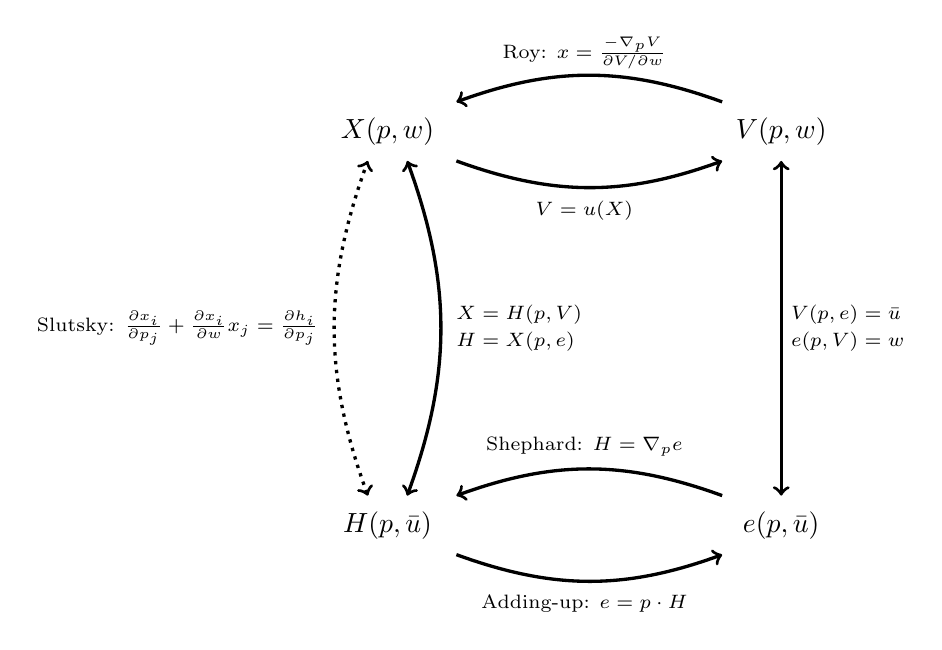
\begin{tikzpicture}[scale=0.5]
		\node at (0,10) {$X(p,w)$};
		\node at (0,0) {$H(p,\bar{u})$};
		\node at (10,0) {$e(p,\bar{u})$};
		\node at (10,10) {$V(p,w)$};
		
		\draw[<->, very thick] (0.5,0.75) to[out=70,in=-70] (0.5,9.25);
		\draw[<->, dotted, very thick] (-0.5,0.75) to[out=110,in=-110] (-0.5,9.25);
		
		\draw[<->,very thick] (10,0.75)--(10,9.25);
		
		\draw[->,very thick] (1.75,-0.75) to[out=-20,in=200](8.5,-0.75);
		\draw[<-,very thick] (1.75,0.75) to[out=20,in=-200](8.5,0.75);
		
		\draw[->,very thick] (1.75,9.25) to[out=-20,in=200](8.5,9.25);
		\draw[<-,very thick] (1.75,10.75) to[out=20,in=-200](8.5,10.75);
		
		\node at (5,2) {\scriptsize Shephard: $H = \nabla_p e$};
		\node at (5,-2) {\scriptsize Adding-up: $e = p \cdot H$};
		\node[right] at (10,5.35) {\scriptsize $V(p,e) = \bar{u}$};
		\node[right] at (10,4.65) {\scriptsize $e(p,V) = w$};
		
		\node[left] at (-1.5,5) {\scriptsize Slutsky: $\frac{\partial x_i}{\partial p_j} + \frac{\partial x_i}{\partial w} x_j = \frac{\partial h_i}{\partial p_j}$};
		\node[right] at (1.5,5.35) {\scriptsize $X = H(p,V)$};
		\node[right] at (1.5,4.65) {\scriptsize $H = X(p,e)$};
		
		\node at (5,12) {\scriptsize Roy: $x = \frac{-\nabla_p V}{\partial V / \partial w}$};
		\node at (5,8) {\scriptsize $V = u(X)$};
	\end{tikzpicture}
	\caption{Relationships Between UMP and EMP}
	\label{fig:ump_emp_relationships}
\end{figure}

\newpage
\section{Producer Theory (Harris)}\label{sec:harris}

\subsection{Classical Producer Theory}

\subsubsection{Setup}

We will always assume the following:

\begin{assumption}
	There are $L$ commodities, with a production plan $y \in \reals^L$. A net input is an element $i$ such that $y_i < 0$, and a net output is an element $j$ such that $y_j > 0$. We have a production possibilities set $Y \subseteq \reals^L$, and we assume that prices $p \ge 0$ that are unaffected by the activity of the firm.
\end{assumption}

We will also often assume, for simplicity (and in order to work with functions rather than correspondences):
\begin{assumption}
	$Y$ is nonempty, closed, and (strictly) convex, and (the \blue{free disposal property}) if $y \in Y$ and $y' \le y$, then $y' \in Y$.
\end{assumption}

\begin{definition}
	A production plan $y \in Y$ is \blue{efficient} if there does not exist $y' \in Y$ such that $y' \ge y$ and $y_i' > y_i$ for some $i$.
\end{definition}

In the case of a single output, we partition $y$ into output $q \in \reals_+$ and inputs $z \in \reals^{L-1}_+$. This allows us to define the following:

\begin{definition}
	The \blue{production function} $f:\reals^{L-1}_+ \to \reals_+$ is defined by 
	\[
	f(x) = \max q \st (q,-z) \in Y
	\]
\end{definition}

\begin{definition}
	The \blue{input requirement set}
	\[
	V(q) \coloneqq \{z \in \reals_+^{L-1} : (q,-z) \in Y\}
	\]
	gives all of the input vectors that can be used to produce an output $q$.
\end{definition}

\begin{definition}
	The \blue{isoquant} 
	\[
	Q(q) \coloneqq \{z \in \reals_+^{L-1} : z \in V(q) \text{ and } z \not\in V(q') \text{ for any } q' > q\}
	\]
	gives all the input vectors that can be used to produce at most $q$ units of output.
\end{definition}

\subsubsection{Cost Minimization}

We will make the following assumptions through this section:

\begin{assumption}
	There are $L-1$ inputs $z$, and one output $q = f(z)$. The production function $f$ is twice continuously differentiable, and inputs have price $w \in \reals^{L-1}_+$
\end{assumption}
\begin{remark}
	If any input has price zero, the firm will obviously not consider it in its decision making.
\end{remark}

\begin{definition}
	The firm's \blue{cost minimization problem} is
	\[
	\min_{z \in \reals^{L-1}_+} w \cdot z \st f(z) = q
	\]
	The associated value function is called the \blue{cost function}
	\[
	C(w,q) \coloneqq \min_{z \in \reals^{L-1}_+} w \cdot z \st f(z) = q
	\]
\end{definition}

\begin{proposition}\label{prop:cost_fn_properties}
	\red{(Properties of the Cost Function)}
	
	\begin{itemize}
		\item[(i)] $C$ is homogeneous of degree 1 in $w$
		\item[(ii)] $C$ is concave in $w$
		\item[(iii)] If we assume free disposal, $C$ is nondecreasing in $q$
		\item[(iv)] If $f$ is homogeneous of degree $k$ in $z$, $C$ is homogeneous of degree $\frac{1}{k}$ in $q$
	\end{itemize}
\end{proposition}
\begin{proof}
	
	\begin{itemize}
		\item[(i)] Increasing $w$ by $\alpha > 0$ is a monotonic transformation and does not affect the choice of $z$, but it does increase $w \cdot z$ by a factor of $\alpha$.
		\item[(ii)] Fix $w,w' \in \reals^{L-1}_+$, and suppose $C(w,q) = w \cdot z$ and $C(w',q) = w' \cdot z'$. Take $\alpha \in [0,1]$ and let $w'' = \alpha w + (1-\alpha)w'$. Then for $z''$ a cost minimizer at $w''$, we have that
		\[
		C(w'',q) = w'' \cdot z'' = \alpha w \cdot z'' + (1-\alpha)w' \cdot z''
		\]
		We also know that $w \cdot z'' \ge C(w,q)$ and $w'\cdot z'' \ge C(w',q)$, so we have that $C(w'',q) \ge \alpha C(w,q) + (1-\alpha)C(w',q)$.
		\item[(iii)] Suppose that $q' > q$. By free disposal, $q$ can be produced using the same input vector used to produce $q'$.
		\item[(iv)] Homogeneity of degree $k$ of $f$ implies that 
		\[
		f(z) = q \Longleftrightarrow \frac{1}{q} f(z) = 1 \Longleftrightarrow f\parl \frac{z}{q^{1/k}}\parr = 1
		\]
		Thus, we get that
		\begin{align*}
			C(w,q) &= \min_{z}w \cdot z \st f\parl \frac{z}{q^{1/k}}\parr = 1 \\
			&= q^{1/k} \min_z w \cdot \frac{z}{q^{1/k}} \st f\parl \frac{z}{q^{1/k}}\parr = 1  \\
			&= q^{1/k} C(w,1)
		\end{align*}
	\end{itemize}
\end{proof}

\subsubsection{Homogeneous Functions (a brief aside)}

\begin{definition}
	A function $f: X \subseteq \reals^n \to \reals$ is \blue{homogeneous of degree $k$} if
	\[
	f(\alpha x) = \alpha^k f(x) \forall \alpha > 0, x \in X
	\]
	where $k$ is a non-negative integer.
\end{definition}
\begin{proposition}
	If a function $f$ is homogeneous of degree $k$, then any of its partial derivatives are homogeneous of degree $k-1$
\end{proposition}
\begin{proof}
	Let $f_i = \frac{\partial f}{\partial x_i}$. We have that
	\[
	f(\alpha x) = \alpha^k f(x) \Longrightarrow \alpha f_i(\alpha x) = \alpha^k f_i(x) \Longrightarrow f_i(\alpha x) = \alpha^{k-1}f_i(x)
	\]
\end{proof}

\begin{proposition}
	\red{(Euler's Formula)} If $f$ is homogeneous of degree $k$ and differentiable, then at any $x$
	\[
	\sum_{i=1}^n \frac{\partial f(x)}{\partial x_i}x_i = kf(x)
	\]
\end{proposition}
\begin{proof}
	Differentiating with respect to $\alpha$ and evaluating at $\alpha = 1$, we get that
	\[
	f(\alpha x) = \alpha^k f(x) \Longrightarrow \sum_{i=1}^n f_i(\alpha x) x_i = k\alpha^{k-1}f(x) \Longrightarrow \sum_{i=1}^n f_i(x)x_i = kf(x)
	\]
\end{proof}

\begin{proposition}
	If the production function $f$ is homogeneous of degree $k$, then
	\[
	\textnormal{MRTS}_{ij}(z) \coloneqq \frac{\frac{\partial f(z)}{\partial z_i}}{\frac{\partial f(z)}{\partial z_j}} = \frac{\frac{\partial f(\alpha z)}{\partial z_i}}{\frac{\partial f(\alpha z)}{\partial z_j}} \eqqcolon \textnormal{MRTS}_{ij}(\alpha z)
	\]
\end{proposition}
\begin{proof}
	\[
	\frac{f_i(\alpha z)}{f_j(\alpha z)} = \frac{\alpha^{k-1}f_i(z)}{\alpha^{k-1}f_j( z)} = \frac{f_i(z)}{f_j(z)}
	\]
\end{proof}

\subsubsection{Profit Maximization}

\begin{definition}
	The firm's \blue{profit maximization problem} is
	\[
	\max_y p \cdot y \st y \in Y
	\]
	The associated value function is called the \blue{profit function}:
	\[
	\pi(p) \coloneqq \max_y p \cdot y \st y \in Y
	\]
\end{definition}

\begin{remark}
	In the single output case, this becomes
	\[
	\pi(p,w) \coloneqq \max_y p f(z) - w \cdot z 
	\]
	Henceforth, we consider only the single output case.
\end{remark}
\begin{remark}
	Note that profit maximization implies cost minimization.
\end{remark}

\begin{proposition}\label{prop:profit_properties}
	\red{(Properties of the Profit Function)}
	\begin{itemize}
		\item[(i)] Homogeneous of degree 1
		\item[(ii)] Nondecreasing in $p$
		\item[(iii)] Nonincreasing in $w$
		\item[(iv)] Convex in $(p,w)$
		\item[(v)] Continuous
	\end{itemize}
\end{proposition}
\begin{proof}
	\begin{itemize}
		\item[(i)] $\max_z \alpha (pf(z) - w\cdot z) = \alpha \max_z pf(z) - w\cdot z$
		\item[(ii)] $p' \ge p \Longrightarrow p' f(z) \ge p f(z) \forall z$
		\item[(iii)] $w' \ge w \Longrightarrow w' \cdot z \ge w \cdot z$
		\item[(iv)] Let $(p'',w'') := \alpha (p,w) + (1-\alpha)(p',w')$ and let $z,z',z''$ be the solution to the profit maximization problem with the corresponding output prices and input price vectors. Then by definition
		\[
		\pi(p,w) = pf(z) - w \cdot z \ge p f(z'') - w \cdot z''
		\]
		\[
		\pi(p',w') = p'f(z) - w' \cdot z \ge p' f(z'') - w' \cdot z''
		\]
		which implies that
		\begin{align*}
		\alpha \pi(p,w) + (1-\alpha)\pi(p',w') &\ge \alpha (p f(z'') - w \cdot z'') + (1-\alpha) ( p' f(z'') - w' \cdot z'') \\
		&= (\alpha p + (1-\alpha)p') f(z'') - (\alpha w + (1-\alpha)w' )\cdot z'' \\
		&= \pi(p'',w'')
		\end{align*}
		\item[(v)] Follows from Berge's Theorem
	\end{itemize}
\end{proof}

\begin{remark}
	$\pi$ being convex in $(p,w)$ implies that $\pi$ is convex in $p$ and $w$ individually.
\end{remark}

\begin{definition}
	The \blue{unconditional input demand function}
	\[
	x(p,w) \coloneqq \argmax_{z \in \reals^{L-1}_+} pf(z) - w\cdot z
	\]
	is the solution to the profit maximization problem. The \blue{output supply function}
	\[
	q(p,w) \coloneqq f(x(p,w))
	\]
	is the output level where the profit is being maximized.
\end{definition}

\begin{proposition}\label{prop:hotelling}
	\red{(Hotelling's Lemma)} If $\pi$ is differentiable, then for $(p,w) \in \reals^L_{++}$,
	\begin{align*}
		q(p,w) &= \frac{\partial \pi(p,w)}{\partial p} \\
		x_j(p,w) &= -\frac{\partial \pi(p,w)}{\partial w_j}
	\end{align*}
\end{proposition}
\begin{proof}
	(Sketch) Apply the Envelope Theorem, and note that $x(p,w)$ is the profit maximizing bundle and $q(p,w)$ is the production function evaluated at that bundle.
\end{proof}

\begin{remark}
	This condition can be relaxed from differentiability to the unconditional input demand function and output supply function being well-defined functions.
\end{remark}

\begin{definition}
	The \blue{conditional input demand function} 
	\[
	z(w,q) \coloneqq \argmin_{z \in \reals^{L-1}_+} w \cdot z \st f(z) = q
	\]
	is the solution to the cost minimization problem.
\end{definition}

\begin{proposition}
	\red{(Shephard's Lemma)} If $C$ is differentiable, then for $w \in \reals^{L-1}_{++}$,
	\[
	z_i(w,q) = \frac{\partial C(w,q)}{\partial w_i}
	\]
\end{proposition}
\begin{proof}
	(Sketch) Similarly, apply the Envelope Theorem to the cost minimization problem.
\end{proof}

\begin{proposition}
	Suppose the profit function is twice continuously differentiable. Then:
	\begin{itemize}
		\item[(i)] $\frac{\partial q(p,w)}{\partial p_i} \ge 0$
		
		\item[(ii)] $\frac{\partial x_j(p,w)}{\partial w_j} \le 0$
		
		\item[(iii)] $\frac{\partial x_j(p,w)}{\partial w_i} = \frac{\partial x_i(p,w)}{\partial w_j}$
	\end{itemize}
\end{proposition}
\begin{proof}
	Note that the profit function being twice continuously differentiable and convex implies that its Hessian is positive semdefinite. Conclusion follows from applying Hotelling's Lemma
\end{proof}

\begin{proposition}
	Suppose the cost function is twice continuously differentiable. Then:
	\begin{itemize}
		\item[(i)] $\frac{\partial z_i(w,q)}{\partial w_i} \le 0$
		
		\item[(ii)] $\frac{\partial z_j(w,q)}{\partial w_i} = \frac{\partial z_i(w,q)}{\partial w_j}$
		
		\item[(iii)] $\frac{\partial z_i(w,q)}{\partial q} = \frac{\partial MC(w,q)}{\partial w_i} = \begin{cases} > 0 & \textnormal{Normal Input} \\ < 0 & \textnormal{Inferior Input} \end{cases}$
	\end{itemize}
\end{proposition}
\begin{proof}
	(i) follows from $C$ being concave in $w$. (ii) and (iii) follow from the symmetry of second derivatives of $C$.
\end{proof}

\subsubsection{Comparative Statics}

\begin{remark}
	For a full treatment, including a few producer theory examples, see Tak's notes on Comparative Statics.
\end{remark}

\begin{assumption}
	Two inputs $(x_1,x_2)$, one output $q = f(x)$. $f \in C^2$ and the Hessian $H_f$ is negative definite. $f(0,x_2) = f(x_1,0) = 0$, so both inputs are necessary. Inada conditions on $x_1,x_2$, output price $p > 0$, input prices $w \gg 0$.
\end{assumption}

Consider the profit maximization problem
\[
\max_{x \in \reals^2_{++}} pf(x) - wx
\]

\begin{exercise}
	Prove that $\partial x_1(p,w) / \partial w_1 < 0$. Taking FOC, we get
	\[
	pf_1(x) - w_1 = 0 \quad \text{ and }\quad pf_2(x) - w_2 = 0
	\]
	We have that the Hessian of $x$, $H_x$, is 
	\[
	H_x = p \matrixc{f_{11} & f_{12} \\ f_{21} & f_{22}} = pH_f
	\]
	Since $H_f$ is negative definite, this matrix is invertible. By the Implicit Function Theorem, FOCs implicitly define $x(p,w) = (x_1(p,w), x_2(p,w))$, and we can rewrite them as
	\[
	pf_1(x(p,w)) - w_1 = 0 \quad \text{ and } \quad pf_2(x(p,w)) - w_2 = 0
	\]
	Taking derivatives with respect to $w_1$, we get
	\[
	pf_{11} \frac{\partial x_1}{\partial w_1} + p f_{12} \frac{\partial x_2}{\partial w_1} = 1
	\]
	\[
	pf_{21} \frac{\partial x_1}{\partial w_1} + p f_{22} \frac{\partial x_2}{\partial w_1} = 0
	\]
	which gives us
	\[
	p \matrixc{f_{11} & f_{12} \\ f_{21} & f_{22}} \matrixc{\partial x_1 / \partial w_1 \\ \partial x_2 / \partial w_1} = \matrixc{1 \\ 0}
	\]
	We get that
	\begin{align*}
	\matrixc{\partial x_1 / \partial w_1 \\ \partial x_2 / \partial w_1} &= \frac{1}{p} \frac{1}{f_{11}f_{22} - f_{12} f_{21}} \matrixc{f_{22} & -f_{12} \\ -f_{21} & f_{11}} \matrixc{1 \\ 0} \\
	&= \frac{1}{p} \frac{1}{f_{11}f_{22} - f_{12} f_{21}} \matrixc{f_{22} \\ -f_{21}}
	\end{align*}
	Note that $f_{11}f_{22} - f_{12}f_{21} > 0$, because $H_f$ is negative definite, and that $f_{22} < 0$, which means that $\frac{\partial x_1}{\partial w_1} < 0$.
\end{exercise}

\begin{question}
	Why is it worth studying cost minimization and profit maximization separately? There are some settings where profit maximization might be unreasonable:
	\begin{itemize}
		\item Dynamics. For example, if there is learning by doing, this gives a firm incentives to choose $q > q(p,w)$ today in order to decrease tomorrow's costs
		\item Managerial utility maximization. If a larger firm gives more prestige, might have $q > q(p,w)$
	\end{itemize}
\end{question}



\subsection{Non-Price-Taking Firms}

In our assumptions, we said that firms were unaffected by the firm's activity. This leads to the simple problem we've been working in:
\[
\max_{z \in \reals^{L-1}} pf(z) - wz
\]
If their output has market power, then we have
\[
\max_{z \in \reals^{L-1}} p(f(z))f(z) - wz
\]
And we assume that $p'(q) < 0 \forall q$. They could also have input market power:
\[
\max_{z \in \reals^{L-1}} pf(z) - w(z)z
\]
where we assume that $\frac{\partial w_i(z)}{\partial z_i} > 0$ and $\frac{\partial w_i(z)}{\partial z_j} = 0 \forall i \ne j$. 


These problems imply that:
\begin{center}
	\begin{tabular}{| c | c | c | c | }
		\hline
		 Statistic & No MP & Output MP & Input MP \\
		 \hline
		 FOCs & $p \nabla f(z) = w$ & $[p(f(z)) + p'(f(z))f(z)] \nabla f(z) = w$ & $p f_i(z) = w_i'(z_i)z_i + w_i(z_i)$\\
		 \hline
		 MRTS & $\frac{f_i(z)}{f_{i'}(z)} = \frac{w_i}{w_{i'}}$ & $\frac{f_i(z)}{f_{i'}(z)} = \frac{w_i}{w_{i'}}$ & $\frac{f_i(z)}{f_{i'}(z)} = \frac{w_i'(z_i)z_i + w_i(z_i)}{w_{i'}'(z_{i'})z_{i'} + w_{i'}(z_{i'})}$\\
		 \hline
	\end{tabular}
\end{center}

We have that profit maximization implies cost minimization in each world, with slight differences. We have that with no market power,
\begin{align*}
	\pi(p,w) &\equiv \max_{z \in \reals^{L-1}} pf(z) - w \cdot z \\
	&= \max_q \barl \max_{z \in \reals^{L-1}} pq - w \cdot z \st f(z) = q \barr \\
	&= \max_q p\cdot q - \barl \min_{z \in \reals^{L-1}} w \cdot z \st f(z) = q \barr \\
	&=  \max_q p\cdot q - C(w,q)
\end{align*}
With output market power, this becomes
\begin{align*}
	\pi(p,w) &\equiv \max_{z \in \reals^{L-1}} p(f(z))f(z) - w \cdot z \\
	&= \max_q \barl \max_{z \in \reals^{L-1}} p(q)q - w \cdot z \st f(z) = q \barr \\
	&= \max_q p(q)\cdot q - \barl \min_{z \in \reals^{L-1}} w \cdot z \st f(z) = q \barr \\
	&=  \max_q p(q)\cdot q - C(w,q)
\end{align*}
With input market power, we have
\begin{align*}
	\pi(p,w) &\equiv \max_{z \in \reals^{L-1}} pf(z) - w(z) \cdot z \\
	&= \max_q \barl \max_{z \in \reals^{L-1}} pq - w(z) \cdot z \st f(z) = q \barr \\
	&= \max_q p\cdot q - \barl \min_{z \in \reals^{L-1}} w(z) \cdot z \st f(z) = q \barr \\
	&=  \max_q p\cdot q - C(q)
\end{align*}

Under perfect competition, there is no profit -- the FOCs imply that
\[
p = \frac{\partial }{\partial q} C(w,q) \text{ \ie, price is marginal cost}
\]
With output market power, we have that
\[
p(q^m) + p'(q^m)q^m = \frac{\partial }{\partial q} C(w,q^m)
\]
which implies that
\[
p(q^m) = \frac{\partial }{\partial q} C(w,q^m) - \underbrace{p'(q^m)}_{<0}q^m > \frac{\partial}{\partial q} C(w,q^m)
\]
so there is positive profit. This with quantity choice. We can equivalently look at the price choice problem. We have
\[
\max_p p D(p) - c(w,D(p)) \Longrightarrow [p^m D'(p^m) + D(p^m)] = \frac{\partial}{\partial q} C(w,D(p^m)) D'(p^m)
\]
which implies that
\begin{align*}
	p^m - \frac{\partial}{\partial q}C(w,q^m) &= -\frac{D(p^m)}{D'(p^m)} \\
	p^m &= \parl \frac{\varepsilon}{1 + \varepsilon}\parr \frac{\partial}{\partial q} C(w,D(p^m))
\end{align*}
where $\varepsilon$ is the negative inverse of the Lerner index.

With input market power (supposing for simplicity that there is only one input), we have
\[
\max_z pf(z) - w(z)z
\]
Since $w(z)$ is increasing, we can write its inverse $z(w)$, and get
\[
\max_w pf(z(w)) - w z(w)
\]
and the FOC get us
\begin{align*}
	p f'(z(w)) z'(w) &= z'(w) w  + z(w) \\
	p \frac{f'(z(w))}{w} &= \frac{z(w)}{z'(w)w} + 1 \\
	p \frac{f'(z(w))}{w} &= \frac{1}{\varepsilon_{z,w}} + 1 = \frac{1 + \varepsilon_{z,w}}{\varepsilon_{z,w}} \\
	w &= \parl \frac{\varepsilon_{z,w}}{1 + \varepsilon_{z,w}} \parr p f'(z(w)) < p f'(z(w))
\end{align*}
where $\varepsilon_{z,w}$ is the elasticity of input supply.

\newpage
\section{Uncertainty Theory (Blume)}\label{sec:blume}

\textbf{\emph{n.b.}} Prof. Blume did not prove any of the results presented here. It clearly matters more that one understands the intuition rather than the exact proof structure. Proof sketches are added wherever possible. I have relied on \href{https://www.semanticscholar.org/paper/Utility-theory-for-decision-making-Fishburn/905a24a912171436e0abd3b5f1fdcb963e6f852f}{Fishburn (1970)} for these proof sketches.

\subsection{Models of Preferences}\label{subsec:models_blume}

\begin{remark}
	There are three main preference models that we will consider here: \href{https://psycnet.apa.org/record/1947-03159-000}{von Neumann and Morgenstern (1947)}, where the objects of choice are probability distributions on outcomes; \href{https://psycnet.apa.org/record/1955-00117-000}{Savage (1954)}, where the objects of choice are outcome-valued random variables (formally, functions from states of the world to outcomes); and \href{https://pages.stern.nyu.edu/~dbackus/Exotic/1Ambiguity/AnscombeAumann\%20AMS\%2063.pdf}{Anscombe and Aumann (1963)}, where the objects of choice are functions from states of the world to probability distributions over outcomes.
\end{remark}

\begin{model}
	\red{von Neumann--Morgenstern} We have $X$ a set of \blue{outcomes} (or prizes) and $P$ the set of probability distributions on $X$, called \blue{lotteries}. For each $p \in P$, we define the \blue{support} of $p$ as
	\[
	\text{supp } p = \{x \in X : p(x) > 0\}
	\]
	A preference relation $\succsim$ on $P$ has an \blue{expected utility representation} if there is a real-valued function $u: X \to \reals$ such that
	\[
	p \succsim q \Longleftrightarrow \sum_{x \in \text{supp } p} u(x)p(x) \ge \sum_{y \in \text{supp } q} u(y)q(y)
	\]
\end{model}

\begin{remark}
	In general, people are inconsistent on what they call $u$. Here, we refer to it as the \blue{Bernoulli Utility Function}, following MWG. Prof. Blume also referred to it as the \blue{payoff function}.
\end{remark}

\begin{remark}
	In this model, whenever $X$ is finite, indifference curves are linear in probabilities. See Figure~\ref{fig:indifference_probability}, where indifference curves are in red.
	
	\begin{figure}[H]
		\centering
		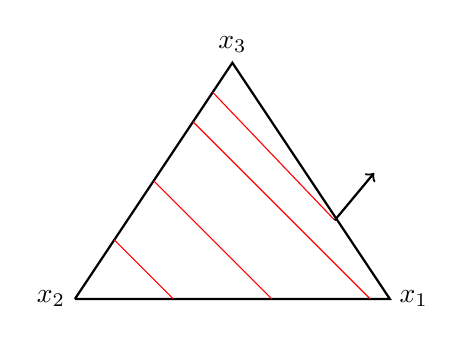
\begin{tikzpicture}[scale=1]
			\draw[thick] (0,0)--(2,3)--(4,0)--(0,0);
			\node[above] at (2,3) {$x_3$};
			\node[right] at (4,0) {$x_1$};
			\node[left] at (0,0) {$x_2$};
			
			\draw[red] (1,1.5)--(2.5,0);
			\draw[red] (0.5,0.75)--(1.25,0);
			\draw[red] (1.5,2.25)--(3.75,0);
			\draw[red] (1.75,2.625)--(3.3,1);
			
			\draw[->,thick] (3.3,1)--(3.8,1.6);
		\end{tikzpicture}
		\caption{Indifference Curves Over Probability Distributions}
		\label{fig:indifference_probability}
	\end{figure}
\end{remark}


\begin{model}
	\red{Savage} We have $X$ a set of outcomes, $S$ a set of \blue{states of the world}, and $F$ the set of \blue{Savage acts}, where $f \in F$ is a function $f : S \to X$. A preference relation $\succsim$ on $F$ has an expected utility representation if there is a probability distribution $p$ on $S$ and a real-valued function $u: X \to \reals$ such that
	\[
	f \succsim g \Longleftrightarrow \sum_{s \in S} u(f(s))p(s) \ge \sum_{s \in S} u(g(s))p(s)
	\]
\end{model}

\begin{model}
	\red{Anscombe--Aumann} We have $X$ a set of outcomes, $S$ a set of states of the world, $P$ the set of probability distributions on $X$, and $A$ the set of \blue{Anscombe--Aumann Acts}, where $a \in A$ is a function $a: S \to P$. A preference relation $\succsim$ on $A$ has an expected utility representation if there is a probability distribution $p$ on $S$ and a real-valued function $u: X \to \reals$ such that
	\[
	a \succsim b \Longleftrightarrow \sum_{s \in S} \sum_{x \in X} u(x) \parl a(s) (x)\parr p(s) \ge \sum_{s \in S} \sum_{x \in X} u(x) \parl b(s) (x)\parr p(s)
	\]
\end{model}

\subsection{von Neumann--Morgenstern}

We first introduce a famous paradox:

\begin{example}
	\red{The St. Petersburg Paradox} A fair coin is tossed until tails appears. How much would you pay for a lottery ticket that paid off $2^n$ dollars if the first tails appears on the $n$th flip? The expected value of this lottery is
	\[
	EV = \frac{1}{2} \cdot 2 + \frac{1}{4}\cdot 4 + \cdots = 1 + 1 + \cdots = \infty
	\]
	However, clearly it's not reasonable to pay a massive amount of money for this lottery ticket. Why is this happening? There are a few explanations, and we'll go through them in this section.
\end{example}

We make the following assumptions on preferences:

\begin{assumption}\label{ass:vnm}
(referred to as the `Finite $X$ Axioms' by Prof. Blume)
	\begin{itemize}
		\item[(i)] $\succsim$ is complete and transitive
		\item[(ii)] (Independence) For all $0 < \alpha \le 1$ and all $r \in P$,
		\[
		p \succsim q \Longleftrightarrow \alpha p + (1-\alpha)r \succsim \alpha 1 + (1-\alpha)r
		\]
		\item[(iii)] (Archimedean) If $p \succ q \succ r$, then there exists $\alpha,\beta \in (0,1)$ such that
		\[
		\alpha p + (1-\alpha) r \succ q \succ \beta p + (1-\beta)r
		\]
	\end{itemize}
\end{assumption}

\begin{theorem}\label{thm:vnm}
	\red{(von-Neumann--Morgenstern Theorem)} If $\succsim$ satisfies Assumptions~\ref{ass:vnm}, then $\succsim$ has an expected utility representation; there is a function $u: X \to \reals$ such that
	\[
	p \succsim q \Longleftrightarrow \sum_{x \in X} u(x)p(x) \ge \sum_{x \in X} u(x)q(x)
	\]
	Furthermore, if $v: X \to \reals$ is another expected utility representation, then there are constants $\alpha > 0$ and $\beta$ such that $v(x) \equiv \alpha u(x) + \beta$.
\end{theorem}
\begin{proof}
	(Very rough sketch) We will define the distance between two lotteries $p$ and $q$ as a function over a subset of a convex cone in an arbitrary metric space, which exists due to the fact that $X$ is finite. This is mathematically tricky, but actually much easier in low-dimensional Euclidean space. You can imagine what's happening by considering the positive-positive quadrant of $\reals^2$, which is a convex cone. From there, the assumptions give us that the cone is convex and compact, and the relationship we are looking for follows directly from the Extreme Value Theorem, considering the roots of the distance function. The second conclusion follows directly from the fact that affine transformations preserve convexity and extrema.
\end{proof}

\begin{definition}
	A \blue{simple lottery} is $p:= (p_1 : x_1,p_2:x_2,\dots,p_K:x_K)$, where $x_1,\dots,x_K$ are outcomes in $\reals$ and $p_1,\dots,p_K$ are probabilities. Let $\mathcal{L}$ denote the set of simple lotteries, and let $u: X \to \reals$ and $U(p) = \sum_{k} u(x_k)p_k$. Formally, this is the expectation of the random variable $u(x)$, itself a function of the random variable $x$, where $x \sim p$.
\end{definition}

\begin{question}
	How do we see that this is linear in lotteries? How do we mix lotteries?
\end{question}

For lotteries with common support, mixing is just the convex combination of the probabilities. But what happens when lotteries have different supports?

\begin{example}
	Consider $p \coloneqq (p_1:x_1,p_2:x_2)$ and $q\coloneqq (q_1:y_1,q_2:y_2,q_3:y_3)$. We can say that
	\[
	p\oplus_\alpha q = (\alpha p_1:x_1, \alpha p_2: x_2,(1-\alpha)q_1:y_1, (1-\alpha)q_2:y_2, (1-\alpha)q_3:y_3)
	\]
	\begin{remark}
		This is \emph{not} a convex combination! It combines objects of different sizes. However, expected utility is still linear:
		\begin{align*}
			U(p \oplus_\alpha q) &= \sum_{k=1}^2 \alpha p_k u(x_k) + \sum_{k=1}^3 (1-\alpha)q_ku(y_k) \\
			&= \alpha \sum_{k=1}^2 p_k u(x_k) +(1-\alpha) \sum_{k=1}^3 q_ku(y_k) \\
			&= \alpha U(p) + (1-\alpha)U(q)
		\end{align*}
	\end{remark}
\end{example}

\begin{definition}
	(From \href{https://www.jstor.org/stable/1905540}{Herstein and Milnor (1953)}) A \blue{mixture space} is a set of objects $\Pi$, with typical elements $\pi,\rho,\mu,\nu$ and a family of functions for $0 \le \alpha \le 1$, $\oplus_\alpha : \Pi \times \Pi \to \Pi$ such that
	\begin{itemize}
		\item[(i)] $\pi \oplus_1 \rho = \pi$
		\item[(ii)] $\pi \oplus_\alpha \rho = \rho \oplus_{1-\alpha} \pi$
		\item[(iii)] $(\pi \oplus_\beta \rho) \oplus_\alpha \rho = \pi \oplus_{\alpha\beta} \rho$
	\end{itemize}
	where $\beta \in [0,1]$.
\end{definition}

Some examples:
\begin{itemize}
	\item Convex sets with the operation of convex combinations
	\item Simple probability distributions on convex sets
	\item $S$ and $X$ are sets, and let $M$ denote the set of functions from $S$ to probability distributions on $X$. The $\oplus_\alpha$ are the (pointwise) convex combinations of these functions
\end{itemize}

We can update Assumptions~\ref{ass:vnm} with the mixture space definitions:
\begin{assumption}\label{ass:vnm_mix}
	(i) remains the same. The others:
	
	\begin{itemize}
		\item[(ii)] (Independence) For all $0 < \alpha \le 1$ and all $r \in P$, $p \succsim q \Longrightarrow p \oplus_\alpha r \succsim q \oplus_\alpha r$
		
		\item[(iii)] (Archimedean) If $p \succ q \succ r$, then there exist $\alpha,\beta \in (0,1)$ such that $p \oplus_\alpha r \succ q \succ p \oplus_\beta r$
	\end{itemize}
\end{assumption}

We can also update Theorem~\ref{thm:vnm} to generalize it:
\begin{theorem}\label{thm:vnm_mix}
	If $M$ is a mixture space and $\succsim$ satisfies Assumptions~\ref{ass:vnm_mix}, then there exists a linear function $U: M \to \reals$. Any other linear representation $V$ is a positive affine transformation of $U$.
\end{theorem}

\paragraph{Some Criticisms.} First, the Archimedean property seems quite odd. What happens if one outcome is infinitely preferred to another?

\begin{example}
	Suppose that we have outcomes $x,y,z$ occurring with probabilities $\rho_x,\rho_y,\rho_z$. Further assume that $x$ is \emph{infinitely better} than $y$ and $z$. We have the following (lexicographic, so rational) preference relation: $(\rho_x,\rho_y,\rho_z) \succ(\rho_x',\rho_y',\rho_z')$ if $\rho_x > \rho_x'$ or if $\rho_x = \rho_x'$ and $\rho_y > \rho_y'$. These preferences lead to a counterexample. Let $p = (1,0,0)$, $r = (0,3/4,1/4)$, and $r = (0,1/4,3/4)$. Then $p \succ q \succ r$. For all $\alpha \in (0,1)$, however,
	\[
	\alpha p + (1-\alpha)r = (\alpha, (1-\alpha)/4,3(1-\alpha)/4) \succ q
	\]
\end{example}
To fix this, we will often assume that $X$ has no infinitely large or small elements.

Another criticism is independence. Are preferences linear in probabilities? The following is another famous paradox:

\begin{example}
	\red{The Allais Paradox} (from \href{https://www.jstor.org/stable/1907921}{Allais (1953)}). Consider the following lotteries:
	\[
	A = \begin{cases}\$1\text{M} & p = 1\end{cases}\qquad B = \begin{cases} \$1\text{M} & p = 0.89 \\ \$5\text{M} & p = 0.10 \\ \$0 & p = 0.01\end{cases}
	\]
	\[
	C = \begin{cases}\$1\text{M} & p = 0.11 \\ \$0 & p = 0.89\end{cases}\qquad D = \begin{cases} \$5\text{M} & p = 0.10 \\  \$0 & p = 0.90\end{cases}
	\]
	Most people prefer $A$ to $B$, and prefer $D$ to $C$. This violates the independence axiom.
\end{example}

This paradox can be resolved by strengthening the Archimedean assumption. This requires some topological considerations beyond this course, but admits an expected utility representation such that $u$ is now bounded and continuous.


\begin{remark}
	Thinking back to the St. Petersburg Paradox, we can now look at some solutions posed.
	\begin{enumerate}
		\item Bernoulli suggested that people tend to disregard small probabilities, rounding them to zero. This became, much later, the foundation of Prospect Theory.
		\item Cramer suggested expected utility, the first time it was used! With some assumptions (mainly, that $u$ must be bounded), this resolves the paradox
	\end{enumerate}
\end{remark}

\subsection{Subjective Probability}

We tend to think of three regimes for where probability comes from:
\begin{enumerate}
	\item \blue{Frequentist}: Probabilities exist, and can in principle be measured by repeated experiments.
	\item \blue{Logical}: Probabilities are the weight that an event happens based on evidence. It essentially generalizes truth from $\{0,1\}$ to $[0,1]$
	\item \blue{Bayesian}: Probability is the degree of belief people have that an event will occur
\end{enumerate}

Before thinking deeply about subjective expected utility theory, we need some mathematical background. Here are presented some definitions and results, without proof.

\begin{definition}
	Suppose that $S$ is finite. Suppose that $\mathcal{S}$ is a collection of subsets of $S$ such that (i) $\emptyset \in \mathcal{S}$, (ii) if $A \in \mathcal{S}$, then $A^c \in \mathcal{S}$, and (iii) if $A,B \in \mathcal{S}$, then $A \cap B \in \mathcal{S}$. $\mathcal{S}$ is a \blue{(Boolean) algebra} of \blue{events}. When $S$ is finite, we can take $\mathcal{S} = 2^S$. When $S = \reals$, we need to take more care.
\end{definition}

\begin{definition}
	A \blue{probability} on $\mathcal{S}$ is a function $p : \mathcal{S} \to [0,1]$ such that (i) $p(\mathcal{S}) = 1$ and (ii) if $A \cap B = \emptyset$, then $p(A \cup B) = p(A) + p(B)$.
\end{definition}
\begin{definition}
	A \blue{qualitative probability} is a binary relation $\sqsubseteq$ on $\mathcal{S}$ such that
	\begin{itemize}
		\item[(i)] $\sqsubseteq$ is complete and transitive
		\item[(ii)] $\mathcal{S} \sqsupset \emptyset$
		\item[(iii)] for all $A \in \mathcal{S}$, $\emptyset \sqsubseteq A \sqsubseteq \mathcal{S}$
		\item[(iv)] If $A,B,C \in \mathcal{S}$ and $A \cap C = B \cap C = \emptyset$, then $A \sqsubseteq B \Longleftrightarrow A \cap C \sqsubseteq B \cap C$
	\end{itemize}
\end{definition}

\begin{definition}
	Let $\mathcal{A} = \{A_1,\dots,A_k\}$ and $\mathcal{B} = \{B_1,\dots,B_k\}$ be lists of events, allowing repetitions. The lists $\mathcal{A}$ and $\mathcal{B}$ are \blue{balanced} if for each state $s \in S$, the number of events containing $s$ in $\mathcal{A}$ equals that in $\mathcal{B}$.
\end{definition}

\begin{assumption}\label{ass:mathprob}
	We have the following:
	
	\begin{itemize}
		\item[(i)] $\succsim$ on $\mathcal{S}$ is complete
		\item[(ii)] (Positivity) for all $A \in \mathcal{S}$, $A \succsim \emptyset$
		\item[(iii)] (Non-triviality) $S \succ \emptyset$
		\item[(iv)] (Finite Cancellation) For all pairs of balanced lists $\mathcal{A}$ and $\mathcal{B}$, if for all $1 \le j \le k-1$, $A_j \succsim B_j$, then $B_k \succsim A_k$.
	\end{itemize}
\end{assumption}
\begin{remark}
	Finite Cencellation implies transitivity. 
\end{remark}

\begin{theorem}
	$\succsim$ satisfies Assumptions~\ref{ass:mathprob} if and only if there is a probability $\rho$ on $\mathcal{S}$ such that $A \succsim B \Longleftrightarrow \rho(A) \ge \rho(B)$ 
\end{theorem}


\subsection{The Savage Framework}

Recall that we are now in the Savage framework, defined in Section~\ref{subsec:models_blume}. First, some definitions:

\begin{definition}
	For an act $h$, define $f \mid_A h$ as getting $f(s)$ for $s \in A$, otherwise getting $h(s)$. Let $xAy$ denote the bet that pays off $x$ on $A$ and $y$ otherwise.
\end{definition}

\begin{definition}
	We say that $f \succsim g$ given $A$, denoted $f \succsim_A g$, if $f'$ and $g'$ are actions such that $f'$ agrees with $f$ on $B$, $g'$ agrees with $g$ on $B$, and $f'$ and $g'$ agree with each other outside of $A$.
\end{definition}

\begin{definition}
	An event $A$ is \blue{null} if for all $f$ and $g$, $f \succsim_A g$.
\end{definition}

\begin{definition}
	Sets are ordered $A \succsim B$ if there are outcomes $x \succ y$ such that $xAy \succsim xBy$.
\end{definition}

Now, we get the Savage Axioms:

\begin{assumption}\label{ass:savage}
	These are:
	
	\begin{itemize}
		\item[(i)] $\succsim$ is complete and transitive
		\item[(ii)] if $f \mid_A h \succ g \mid_A h$, then for all $k$, $f \mid_A k \succ g \mid_Ak$
		\item[(iii)] For outcomes $x,y$ and non-null $A$, $x \succsim_A y$ if and only if $x \succsim y$
		\item[(iv)] For outcomes $x \succ y$ and $x' \succ y'$, and sets $A,B$, $xAy \succsim xBy$ if and only if $x' A y' \succsim x' B y'$
		\item[(v)] There exist outcomes $x \succ y$
		\item[(vi)] If $f \succ g$, then for any consequence $x$ there is a partition of $S$ such that on each $S_i$, $f \mid_{S_i} h \succ g$ and $f \succ g \mid_{S_i} h$
		\item[(vii)] If $f$ and $g$ are acts and $A$ is an event such that $f(s) \succsim_A g$ for every $s \in A$, then $f\succsim_A g$; and if $f \succsim_A g(s)$ for every $s \in A$, then $f \succsim_B g$
	\end{itemize}
\end{assumption}

\begin{theorem}
	The Savage Axioms (Assumptions~\ref{ass:savage}) imply Bayes' Rule
\end{theorem}
\begin{proof}
	From the assumptions, $f \succ_A g$ if and only if for any act $h$, $f \mid_A h \succ g\mid_A h$. We have that
	\begin{align*}
		\expect_\mu \barl u(f\mid_A h)\barr &> \expect_\mu\barl u(g \mid_A h)\barr &&\Longleftrightarrow \\
		\int_S u(f \mid_A h(s)) d\mu &> \int_S u(f \mid_A g(s)) d\mu &&\Longleftrightarrow \\
		\int_A u(f(s))d\mu + \int_{A^c} u(h(s))d\mu &> \int_A u(g(s))d\mu + \int_{A^c} u(h(s))d\mu &&\Longleftrightarrow \\
		\int_A u(f(s))d\mu &> \int_A u(g(s))d\mu &&\Longleftrightarrow \\
		\int_A u(f(s))d\mu/\mu(A) &> \int_A u(g(s))d\mu/\mu(A) \\
		\expect_\mu\barl u(f) \mid A\barr &> \expect_\mu\barl u(g) \mid A\barr
	\end{align*}
\end{proof}

\subsection{Anscombe--Aumann}

\begin{remark}
	Recall that we are now in the Anscombe--Aumann framework detailed in Section~\ref{subsec:models_blume}, meaning that an expected utility representation is a function $u: X \to \reals$ and a probability distribution $\mu$ on $S$ such that
	\[
	f \succsim g \Longleftrightarrow \sum_S \sum_X u(x) f(s)(x) \mu(s) \ge \sum_S \sum_X u(x) g(s)(x) \mu(s) 
	\]
\end{remark}

To go towards an expected utility representation theorem, we need some further assumptions, beyond Assumptions~\ref{ass:vnm}.

\begin{assumption}\label{ass:aa}
	In addition to Assumptions~\ref{ass:vnm}, we assume that
	
	\begin{itemize}
		\item[(iv)] (non-triviality) For some $f,g \in A$, $f \succ g$
		\item[(v)] (state independence) If for some $s \in S$, $a \in A$, and $p,q \in P$, $h\mid_{\{s\}^c}p \succ p \succ h\mid_{\{s\}^c}q$, then for all non-null states $t$, $h \mid_{\{s\}^c} p \succ h \mid_{\{s\}^c} q$
	\end{itemize}
\end{assumption}

\begin{theorem}
	If $\succsim$ satisfies Assumptions~\ref{ass:vnm} and Assumptions~\ref{ass:aa}, then there exists a function $u: X \to \reals$ and a probability distribution $\rho$ on $S$ such that
	\[
	f \succsim g \Longleftrightarrow \sum_S \sum_X u(x) f(s)(x) \rho(s) \ge \sum_S \sum_X u(x) g(s)(x) \rho(s)
	\]
\end{theorem}
\begin{proof}
	Complicated, and ommitted. Is in \href{https://www.semanticscholar.org/paper/Utility-theory-for-decision-making-Fishburn/905a24a912171436e0abd3b5f1fdcb963e6f852f}{Fishburn (1970)}.
\end{proof}

\subsection{Beyond Expected Utility}

\begin{remark}
	There are some big issues with expected utility theory in general. Here, some of them are summarized and some possible solutions are presented.
\end{remark}

Consider first a final famous paradox:

\begin{example}
	\red{The Ellsberg Paradox} (from \href{https://www.jstor.org/stable/1884324}{Ellsberg (1961)}) There is a single urn with three balls. One ball is red and the other two are either blue or green. One ball is drawn from the urn, and the bettor bets on its color. Winning bets pay \$100, losing bets pay nothing. Available bets are red, blue, not red, and not blue. 
	
	Typical laboratory preferences are inconsistent with probabilistic beliefs -- both red and not red are preferred to blue and not blue. This is a major issue, with several proposed solutions over the years.
\end{example}

\begin{example}
	Weighted EU. One idea is that individuals overweight small-probability events. Imagine a weighting function $w: [0,1] \to [0,1]$ with $w(p) > p$ for small $p$ and $w(p) < p$ for large $p$. One issue: weighted expected utility will not respect FOSD. 
\end{example}

\begin{example}
	Rank-Dependent Expected Utility. Instead of weighing probabilities, apply probability weights to the CDF:
	\[
	U(p) = \sum_n w_n(p)u(x_n)
	\]
	where $x_1 \le x_2 \le \cdots \le x_n$ and 
	\[
	w_n(p) = q\parl \sum_{k=1}^n p_k\parr - q\parl \sum_{k=1}^{n-1}p_k\parr
	\]
	where $q: [0,1] \to [0,1]$ transforms probabilities and $q(0) = 0 = 1-q(1)$. If $q$ is strictly increasing, than $\succsim$ respects FOSD.
\end{example}

\begin{example}
	Maxmin EU. Ambiguity is the idea that individuals may be uncertain about what probability distribution they face. If, for example, you bet as if the worse case scenario were always the probability distribution for the current bet, the Ellsberg paradox would result.
\end{example}

\begin{definition}
	\blue{Choquet Expected Utility} is expected utility where the expectation is taken with respect to a non-additive probability, also called a \blue{capacity}. Suppose $S$ is finite and $\mathcal{S} = 2^S$. A function $\mu: S \to [0,1]$ is a capacity if (i) $\mu(\emptyset) = 0$, $\mu(S) = 1$, and for all $A \subset B \in S$, $\mu(B) \ge \mu(A)$. 
\end{definition}

\begin{assumption}\label{ass:choquet}
	We have the following assumptions for Choquet Expected Utility over Anscombe--Aumann acts:
	\begin{itemize}
		\item[(i)] $\succsim$ is complete and transitive
		\item[(ii)] An Archimedean axiom
		\item[(iii)] The independence axioms for all acts $f,g,h$ which are comonotonic
		\item[(iv)] There are $f,g \in A$ such that $f \succ g$
		\item[(v)] If for all $s \in S$, $f(s) \succ g(s)$, then $f \succ g$
	\end{itemize}
\end{assumption}

\begin{theorem}
	If $\succsim$ on $A$ satisfies Assumptions~\ref{ass:choquet}, then there is a function $u: X \to \reals$ and a capacity $\mu$ on $S$ such that
	\[
	f \succsim g \Longleftrightarrow \int \sum_x u(x)f(s)(x)d\mu \ge \int \sum_x u(x)g(s)(x)d\mu
	\]
\end{theorem}
\begin{proof}
	Technical, ommitted.
\end{proof}

\begin{definition}
	A capacity $\mu$ is \blue{convex} if for all $A,B \in \mathcal{S}$,
	\[
	\mu(A \cup B) - \mu(A) \ge \mu(B) - \mu(A \cap B)
	\]
	The \blue{core} of a capacity $\mu$ is $C(\mu) \coloneqq \{\rho \in P : \rho(A) \ge \mu(A)\}$
\end{definition}
\begin{lemma}
	Every convex capacity has a core.
\end{lemma}
\begin{example}
	If $S = \{0,1\}$ and $\mu(0) = \mu(1) = 0.3$, then
	\[
	C(\mu) = \{\rho : 0.3 \le \rho(0) \le 0.7\}
	\]
\end{example}
\begin{remark}
	If $P$ is a convex set of probability distributions, then $\mu(A) = \inf_{\rho \in P}\rho(A)$ is a capacity
\end{remark}

\begin{definition}
	Let $\succsim$ be a binary relation on $A$. Then $\succsim$ is said to be \blue{ambiguity-averse} (also called \blue{uncertainty-averse}) if $f,g \succsim h$ and $\alpha \in [0,1]$ implies that $\alpha f + (1-\alpha)g \succsim h$
\end{definition}

\begin{theorem}
	Suppose that $\succsim$ satisfies Assumptions~\ref{ass:choquet}. Then the following are equivalent:
	\begin{enumerate}
		\item $\succsim$ is ambiguity-averse
		\item $\mu$ is convex
		\item $\int f d\mu = \inf_{\rho \in C(\mu)} \int f d\rho$
	\end{enumerate}
\end{theorem}
\begin{remark}
	This is a characterization of maxmin expected utility. Can you see how to obtain the Ellsberg Paradox from this characterization?
\end{remark}







\newpage
\section{Uncertainty Applications (Barseghyan)}\label{sec:barseghyan}

\newpage
\section{Information Theory (Battaglini)}\label{sec:battaglini}

\subsection{Asymmetric Information}

\begin{definition}
	We say that we have \blue{complete information} if all agents know all of the relevant information. We say that information is \blue{incomplete} otherwise. We have two types of incomplete information:
	\begin{itemize}
		\item[(i)] \blue{Symmetric incomplete information}: some variables are unknown, but no privileged information
		\item[(ii)] \blue{Asymmetric incomplete information}: some players have more information than others
	\end{itemize}
\end{definition}

\begin{remark}
	We have two broad categories of asymmetric information problems: (i) \blue{adverse selection}, when the asymmetric information concerns the characteristics of the agents (think insurance, lending, selling, etc); and (ii) \blue{moral hazard} when the information concerns the action of some character (think work relations, also insurance, also lending, etc).
\end{remark}

\begin{model}
	\red{(Lemons)} (from \href{https://www.jstor.org/stable/1879431}{Akerlof (1970)}). Consider a labor market in which a worker produces $\theta$ units. $\theta$ has distribution $F(\theta)$ in $[\underline{\theta},\overline{\theta}]$, with $0 < \underline{\theta} < \overline{\theta} < \infty$. Firms hire workers to produce the good and sell it in a competitive market at price $p = 1$. The number of workers is $N$, and firms are risk-neutral. Workers have a reservation value for their time $r(\theta)$, which can be thought of as unemployment insurance, or the value of going to school, or whatever. Employed workers receive a wage, which may or may not depend on $\theta$.
\end{model}

\paragraph{Complete Information.} In a competitive equilibrium with complete information, all workers with $r(\theta) < \theta$ are employed. $w(\theta) = \theta$ for all employed workers, and $w(\theta) < \theta$ for the unemployed. Note that this market outcome is Pareto optimal: it is not possible to make any worker strictly better off without making some agent strictly worse off. Aggregate surplus in this model is:
\[
W\opt = \int_{\underline{\theta}}^{\overline{\theta}} N \barl \ones_{\theta} \cdot \theta + (1 - \ones_\theta) r(\theta)\barr dF(\theta)
\]
where $\ones_\theta = 1$ if $r(\theta) < \theta$ and 0 otherwise.

\paragraph{Asymmetric Information.} Since worker types are unobservable, there will only be one market here, with price $w$. Supply in this market is $\Theta(w)\coloneqq \{\theta : r(\theta) < w\}$, so $S(w) = F(r^{-1}(w))$. For simplicity, let's assume that indifferent workers will choose to work. Demand is:
\[
D(w) = \begin{cases} 0 & \expect \theta < w \\ [0,\infty] & \expect \theta = w \\ \infty & \expect \theta > w \end{cases}
\]
It is clear that $S(w) = D(w)$ only when $\expect \theta = w$. At the same time, $\expect\theta$ must be consistent with supply, so we must have that $w = \expect\barl\theta : r(\theta) \le w\barr$. This condition is called \blue{rational expectations}.

\begin{definition}
	Ina. competitive market model with unobservable worker's productivity, a \blue{competitive equilibrium} is a wage rate $w\opt$ and a set of workers $\Theta\opt$ such that
	\[
	\Theta\opt = \{\theta : r(w) \le w\} \quad \text{ and } \quad w\opt = \expect\barl \theta : \theta \in \Theta\opt\barr 
	\]
\end{definition}

\begin{remark}
	The rational expectation requirement is well-defined only if $\Theta\opt$ is non-empty. If $\Theta\opt$ is an empty set, we need to specify off-path beliefs, since the firms expect no supply of labor. For now, we have the following, which is as good as anything else:
\end{remark}
\begin{assumption}
	If $\Theta\opt = \emptyset$, then $w\opt = \expect \theta$, the unconditional expectation.
\end{assumption}

\begin{remark}
	In general, with imperfect information, a competitive equilibrium is Pareto inefficient. 
\end{remark}

\begin{example}
	To see this point, assume $r(\theta) = r$ for some constant. The Pareto optimal allocation requires that all workers with $\theta > r$ to work, and all types with $\theta < r$ to not work. But this is impossibly in a competitive equilibrium: if $w > r$, everyone works, and if $w < r$, nobody works. If $w = r$, the types are indifferent, but there's no reason they should sort the way we want. The problem is that firms are unable to distinguish types, so there's no way to sort the workers.
\end{example}


\begin{example}
	(Adverse Selection and Market Unraveling) We now consider the more realistic case where $r(\theta)$ is increasing in $\theta$. For simplicity, we assume that $r(\theta) \le \theta$ for all $\theta$, so it is efficient to have full employment. Further, we assume that $r(\theta)$ is \emph{strictly} increasing in $\theta$. Now we have that $\expect[\theta : r(\theta) \le w]$ is continuous in $w$, as long as $F$ has a density $f$, and is increasing in $w$.
	
	Note some implications: (i) $\expect[\theta : r(\theta) \le r(\underline{\theta})] = \underline{\theta} \ge r(\underline{\theta})$, and (ii) $\expect[\theta : r(\theta) \le r(\overline{\theta})] = \expect \theta < \overline{\theta}$. Thus, we have Figure~\ref{fig:lemon_one_equilibrium}, where $\expect[\theta : r(\theta) \le w]$ is above the $45^\circ$ line at $w = r(\underline{\theta})$, and below at $w = r(\overline{\theta})$. 
	\begin{figure}[H]
		\centering
		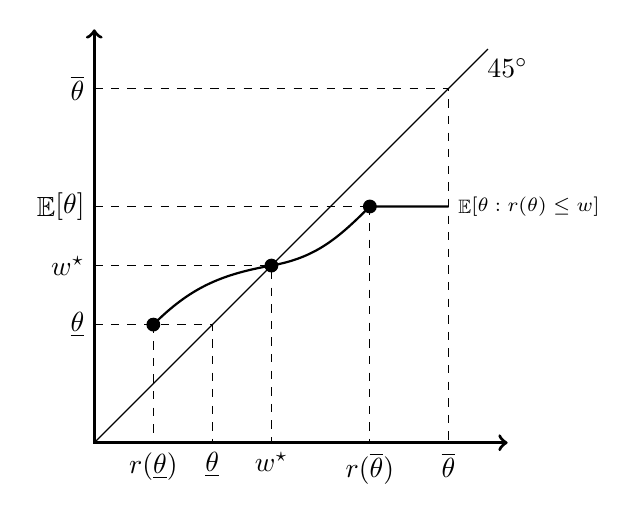
\begin{tikzpicture}[scale=0.5]
    		\draw[very thick,<->] (10.5,0)--(0,0)--(0,10.5);
    		\draw[] (0,0)--(10,10);
 			\node[below] at (10.5,10) {$45^\circ$};   		
    		\draw[dashed] (0,9)--(9,9)--(9,0);
    		\node[left] at (0,9) {$\overline{\theta}$};
    		\node[below] at (9,0) {$\overline{\theta}$};
    		\node[below] at (1.5,0) {$r(\underline{\theta})$};
			\node[below] at (3,0) {$\underline{\theta}$};
			\node[below] at (4.5,0) {$w\opt$};
			\node[below] at (7,0) {$r(\overline{\theta})$};
			\node[left] at (0,6) {$\expect[\theta]$};
			\node[left] at (0,4.5) {$w\opt$};
			\node[left] at (0,3) {$\underline{\theta}$};
			
			\draw[dashed] (0,3)--(3,3)--(3,0);
			\draw[dashed] (0,4.5)--(4.5,4.5)--(4.5,0);
			\draw[dashed] (1.5,3)--(1.5,0);
			\draw[dashed] (0,6)--(9,6);
			\draw[dashed] (7,6)--(7,0);
			
			\draw[thick] (1.5,3) to[out=45, in=190] (4.5,4.5) to[out=10,in=225] (7,6) -- (9,6);
			
			\fill[black] (1.5,3) circle (5pt);
			\fill[black] (4.5,4.5) circle (5pt);
			\fill[black] (7,6) circle (5pt);
			
			\node[right] at (9,6) {\scriptsize $\expect[\theta : r(\theta) \le w]$};
		\end{tikzpicture}
		\caption{Single Equilibrium}
		\label{fig:lemon_one_equilibrium}
	\end{figure}
	
	We must have at least one $w\opt \in (\underline{\theta},\overline{\theta})$ such that $w\opt = \expect[\theta : r(\theta) \le w\opt]$, by Kakutani's Fixed Point Theorem. 
	
	This characterization immediately shows that the equilibrium is inefficient. It would be optimal to have all types employed, but only types $\theta \le r^{-1}(w\opt) < \overline{\theta}$ are employed here. 
\end{example}

\begin{remark}
	We may have multiple equilibria. See Figure~\ref{fig:lemon_multiple_equilibria} for an illustration. If we have multiple equilibria, they can be Pareto ranked -- recall that all profits are zero, but workers do better as $w\opt$ increases.
\end{remark}

\begin{figure}[H]
		\centering
		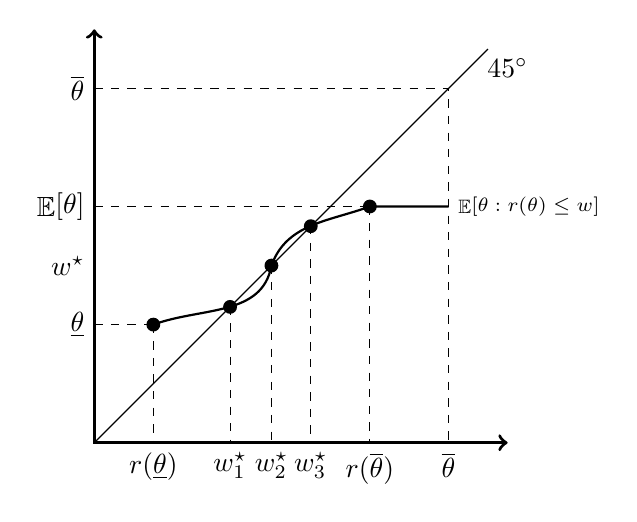
\begin{tikzpicture}[scale=0.5]
    		\draw[very thick,<->] (10.5,0)--(0,0)--(0,10.5);
    		\draw[] (0,0)--(10,10);
 			\node[below] at (10.5,10) {$45^\circ$};   		
    		\draw[dashed] (0,9)--(9,9)--(9,0);
    		\node[left] at (0,9) {$\overline{\theta}$};
    		\node[below] at (9,0) {$\overline{\theta}$};
    		\node[below] at (1.5,0) {$r(\underline{\theta})$};
			\node[below] at (7,0) {$r(\overline{\theta})$};
			\node[left] at (0,6) {$\expect[\theta]$};
			\node[left] at (0,4.5) {$w\opt$};
			\node[left] at (0,3) {$\underline{\theta}$};
			\node[below] at (3.45,0) {$w\opt_1$};
			\node[below] at (4.5,0) {$w\opt_2$};
			\node[below] at (5.5,0) {$w\opt_3$};
			
			\draw[dashed] (0,3)--(1.5,3);

			\draw[dashed] (1.5,3)--(1.5,0);
			\draw[dashed] (0,6)--(9,6);
			\draw[dashed] (7,6)--(7,0);
			\draw[dashed] (3.45,3.45)--(3.45,0);
			\draw[dashed] (4.5,4.5)--(4.5,0);
			\draw[dashed] (5.5,5.5)--(5.5,0);
			
			\draw[thick] (1.5,3) to[out=20, in=-100] (4.5,4.5) to[out=70,in=200] (7,6) -- (9,6);
			
			\fill[black] (1.5,3) circle (5pt);
			\fill[black] (4.5,4.5) circle (5pt);
			\fill[black] (7,6) circle (5pt);
			\fill[black] (3.45,3.45) circle (5pt);
			\fill[black] (5.5,5.5) circle (5pt);
			
			\node[right] at (9,6) {\scriptsize $\expect[\theta : r(\theta) \le w]$};
		\end{tikzpicture}
		\caption{Multiple Equilibria}
		\label{fig:lemon_multiple_equilibria}
	\end{figure}

\begin{remark}
	The classic point made by Akerlof is that the market may totally collapse. See the following example.
\end{remark}

\begin{example}
	Assume that $r(\theta) = \alpha \theta$ for some $\alpha < 1$, and that $\theta \sim U[0,2]$. We have that
	\[
	\expect[\theta : r(\theta) \le w] = \expect[\theta : \alpha \theta \le w] = \expect\barl\theta : \theta \le \frac{w}{\alpha}\barr = \frac{w}{2\alpha}
	\]
	In this case, when $\alpha > \frac{1}{2}$, the market collapses to zero. See Figure~\ref{fig:lemon_collapse}.
	
	\begin{figure}[ht]
		\centering
		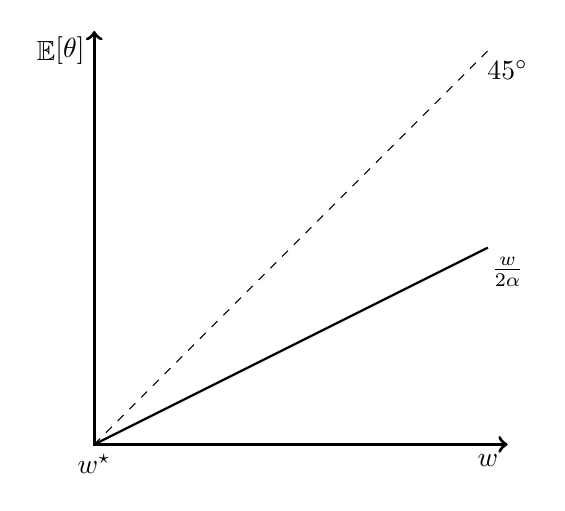
\begin{tikzpicture}[scale = 0.5]
			\draw[<->,very thick] (10.5,0)--(0,0)--(0,10.5);
			
			\draw[dashed] (0,0)--(10,10);
			\draw[thick] (0,0)--(10,5);
			\node[below] at (10,0) {$w$};
			\node[left] at (0,10) {$\expect[\theta]$};
			\node[below] at (10.5,10) {$45^\circ$};
			\node[below] at (10.5,5) {$\frac{w}{2\alpha}$};
			\node[below] at (0,0) {$w\opt$};
		\end{tikzpicture}
		\caption{Collapse In the Market for Lemons}
		\label{fig:lemon_collapse}
	\end{figure}
\end{example}

\begin{question}
	Could this be fixed with public intervention? A case is possible where there are multiple equilibria. In this case, the government could shift the equilibrium to the maximum equilibrium wage. 
	
	Could the government do better than that? If they could see the types, but that's implausible.
\end{question}
\begin{definition}
	A \blue{Constrained Pareto Optimum} is a Pareto Optimum achievable by a planner with no informational advantage. 
\end{definition}
Is there a constrained Pareto optimum that is better than the competitive equilibrium? The answer is no.

\begin{example}
	The planner chooses $w_e$ and $w_u$ (employed and unemployed). Given this, all workers of type $\theta \le \hat{\theta}$ will work, where $w_u + r(\hat{\theta}) = w_e$. So the government can only choose $\hat{\theta}$, $w_e$, and $w_u$ such that the budget balance is satisfied:
	\[
	w_e F(\hat{\theta}) + w_u [ 1 - F(\hat{\theta})] \le \int \theta dF(\theta)
	\]
	Substituting, we get that
	\begin{align*}
		w_u(\hat{\theta}) &= \int \theta dF(\theta) - r(\hat{\theta})F(\hat{\theta}) \\
		w_e(\hat{\theta}) &= \int \theta dF(\theta) - r(\hat{\theta})[1-F(\hat{\theta})]
	\end{align*}
	meaning that
	\begin{align*}
		w_u(\hat{\theta}) &=F(\hat{\theta}) \barl \expect [\theta : \theta \le \hat{\theta}] - r(\hat{\theta})\barr \\
		w_e(\hat{\theta}) &= F(\hat{\theta}) \barl \expect [\theta : \theta \le \hat{\theta}] - r(\hat{\theta})\barr + r(\hat{\theta})
	\end{align*}
	Let $\theta\opt$ be the highest type employed in the highest competitive equilibrium, so:
	\[
	r(\theta\opt) \expect[\theta : \theta \le \theta\opt] = w\opt
	\]
	If the government selects $\hat{\theta} = \theta\opt$, we have $w_e(\hat{\theta}) = w\opt$, and $w_u(\hat{\theta}) = 0$. So the outcome is the competitive equilibrium. There are two other possibilities: $\hat{\theta} > \theta\opt$ and $\hat{\theta} < \theta\opt$. If $\hat{\theta} < \theta\opt$, we have that
	\[
	w_e(\hat{\theta}) = F(\hat{\theta}) \barl \expect [\theta : \theta \le \hat{\theta}] - r(\hat{\theta})\barr + r(\hat{\theta})
	\]
	\[
	\qquad\quad< F(\hat{\theta}) \barl \expect [\theta : \theta \le \hat{\theta}] - r(\theta\opt)\barr + r(\theta\opt)
	\]
	since $r(\theta\opt) > r(\hat{\theta})$. We also have that
	\begin{align*}
		w_e(\hat{\theta}) - r(\theta\opt) &\le F(\hat{\theta})\barl \expect[\theta : \theta \le \hat{\theta}] - r(\theta\opt)\barr \\
		&= F(\hat{\theta})\barl \expect[\theta : \theta \le \hat{\theta}] -\expect[\theta : \theta \le \theta\opt]\barr < 0
	\end{align*}
	It follows directly that $w_e(\hat{\theta}) < r(\theta\opt) = w\opt$. Low types were working in the competitive equilibrium for a higher wage, and they are now worse off.
	
	The other case assumes that $\hat{\theta} > \theta\opt$. We must have that $\expect[\theta : r(\theta) \le w] < w$ for all $w \ge w\opt$, otherwise $w\opt$ would not be the highest competitive equilibrium. Since $w\opt = r(\theta\opt)$ and $r(\theta)$ is increasing, $r(\hat{\theta}) > r(\theta\opt) = w\opt$, so
	\[
	\expect\barl \theta : r(\theta) \le r(\hat{\theta})\barr < r(\hat{\theta})
	\]
	for $\hat{\theta} \ge \theta\opt$. So $w_u(\hat{\theta}) = F(\hat{\theta}) \barl \expect[\theta : \theta \le \hat{\theta}] - r(\hat{\theta})\barr \le 0$, implying that the high types that remain unemployed are worse off now.
\end{example}

\begin{example}
	One way the market might bypass the information asymmetry is by allowing workers to signal their type. Assume here that there are two types, $0 < \theta_L < \theta_H$, with $\prob\{\theta_H\} = \lambda$. We now assume that workers can get some education $e$. To make the point more striking, education is unproductive. 
\end{example}

\newpage
\section{Exercises and Examples}\label{sec:exercises}

\subsection{Choice (Easley)}

\subsubsection{Easley Homework}

\subsubsection{TA Section Examples}

\subsubsection{Outside Questions}

\subsection{Consumer (Kircher)}

\subsubsection{Kircher Homework}

\subsubsection{TA Section Examples}

\subsubsection{Outside Questions}

\subsection{Producer (Harris)}

\subsubsection{Harris Homework}

\subsubsection{TA Section Examples}

\subsubsection{Outside Questions}

\subsection{Uncertainty (Blume)}

\subsubsection{Blume Homework}

\subsubsection{TA Section Examples}

\subsubsection{Outside Questions}

\subsection{Uncertainty (Barseghyan)}

\subsubsection{Barseghyan Homework}

\subsubsection{TA Section Examples}

\subsubsection{Outside Questions}

\subsection{Information (Battaglini)}

\subsubsection{Battaglini Homework}

\subsubsection{TA Section Examples}

\subsubsection{Outside Questions}












\end{document}